%\chapter{As light as a feather}
\chapter{ILD vertex detector and PLUME project}
\label{chap:vxd}
  
  Since the end of the 1960's, the development of position sensitive silicon sensors has permitted the confirmation of the predictions of the \acrfull{SM} with a high precision, as well as the discovery of the top quark.
  These sensors, mostly employed for the \acrfull{VXD}, are used to track the particles down to their decay vertices.
  The design of such a device is driven by the physics requirement of the experiment and plays a crucial role at the \acrfull{ILC}.
  For example, one flagship measurement is the study of the Higgs boson couplings to fermions and other bosons.
  This can be achieved only with precise heavy flavor tagging and the ability to separate the $b$ quarks from the $c$ quarks. 
  Actually, the lifetime of the two quarks is of the same magnitude ($1.3 \cdot 10^{-12}~\rm{s}$ for the $b$ quark and $1.1 \cdot 10^{-12}~\rm{s}$ for the $c$ quark), leading to very close decay vertices. 
  
  In this chapter, the role of the vertex detector and the physics requirements to develop one for the \gls{ILC} environment will be presented.
  Then, the different options of the \acrfull{ILD} are shown.
  The double-sided ladders developed by the \gls{PLUME} collaboration are presented.
  To finish, the principle of \gls{CMOS} sensors and their use in physics are described.

  \minitoc
  
  \section{The ILD vertex detector specifications}
   
    The \gls{VXD} is the sub-detector closest to the \acrfull{IP}.
    It is in charge of reconstructing the vertex by extrapolating particles back to their origin. 
    This detector should be optimised to track particles in a high-density environment, especially those originating from the decay of the $B$ and $C$-mesons.
    The reconstruction of displaced vertices should be efficient enough to perform good flavour tagging.
    Therefore, the detector has to measure particles with a lifetime in the picosecond regime, representing a decay length between 150 and $500~\rm{\mu m}$.
    The minimum distance of the first \gls{VXD} layer to the \gls{IP} is determined by the beam pipe radius and the background induced by beamstrahlung, to limit the pixel occupancy.
    Depending on the option chosen (see section~\ref{subsec:layout}), the \gls{VXD} has to provide five or six points of measurement with a very precise spatial resolution.
    For the studies requiring vertex charge reconstruction, the \gls{VXD} should be able to reconstruct low-momentum and very forward tracks.

    \begin{figure}[!tbh]
      \centering
      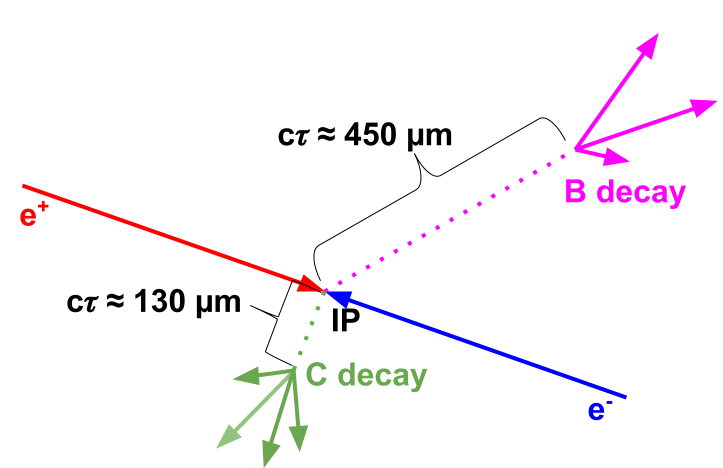
\includegraphics[width = 0.8\textwidth]{Pictures/Higgs/ImpactParameter.png}
      \caption{Scheme of the vertex detector impact parameter. To distinguish $B$-meson and $C$-meson decays, the innermost layer has to be as close as possible to the interaction point. The next layer has to be farer to it.}
      \label{fig:IP}
    \end{figure}

   \subsection{Performance requirements}
   
   The ideal \gls{VXD} should be made of sensors with a fine granularity in order to increase the ability to locate precisely the particle impacts and to distinguish two nearest particles.
   The mechanical structure of the detector should provide a good stiffness and stability of the whole system but has to be, at the same time, as light as possible to reduce the interaction of the particles traversing it, before they reached another part of the main detector.
   Also, in order to reduce the unwanted interactions, the sensor technology used has to have a low power consumption to avoid any special cooling system which can have a negative impact on the material budget.
   The design of such a detector, like the minimal distance of the first layer to the \gls{IP} and the spacing between different layers, is determined by both the beam background and the physics to study.
   Figure~\ref{fig:IP} represents the impact parameter of a vertex detector.
   To distinguish $B$-meson decay from $C$-meson decay, the innermost layer has to be as close as possible to the \gls{IP}, whereas the outer-layer has to be as far as possible.
   The flavour tagging ability, the vertex charge measurement and tracking, and the displaced vertices reconstruction are the main physics parameters driving the design.
   The distance of closest approach of a particle to the collision point is called the impact parameter and the resolution achievable by the detector can be approximated with formula~\ref{eq:resIP}~\cite{Battaglia2011}.
    
    \begin{equation}
      \sigma_{IP} = a \oplus \frac{b}{p \sin{\theta}^{k}}~\rm{,~with~k~=}
      \left\{
        \begin{array}{r l}
          \frac{3}{2} & \text{in the } R - \Phi \text{ projection,} \\
          \frac{5}{2} & \text{in the z projection.}
        \end{array}
      \right. 
      \label{eq:resIP}
    \end{equation}

    Where $\theta$ is the track polar angle (\gls{ILD} coordinate systems are presented in section~\ref{sec:ILD}), $a$ and $b$ are explained in the following way.

   The first term $a$ is the impact parameter resolution of the sensors used for the \gls{VXD}, which is related to the radius of the inner $R_{\rm{int}}$ and outer $R_{\rm{ext}}$ layers and the single point resolution $\sigma_{s.p.}$, as described in equation~\ref{eq:aTerm}.

   \begin{equation}
     a = \sigma_{s.p} \cdot \frac{R_{\rm{int}} \oplus R_{\rm{ext}}}{R_{\rm{ext}} - R_{\rm{int}}}.
     \label{eq:aTerm}
   \end{equation}

  In the case of \gls{ILD}, the single point resolution should not be higher than $\sigma_{sp} \simeq 3~\rm{\mu m}$, leading to an impact parameter with a resolution of the order of $a \simeq 5~\rm{\mu m}$.
  
  The second term, $b$, presented in equation~\ref{eq:bTerm}, is related to the multiple scattering introducing an uncertainty on the impact parameter.
  
  \begin{equation}
    b = R_{int} \frac{13.6 MeV/c}{\beta c} \cdot Z \cdot \sqrt{\frac{x}{X_{0}}} \left[ 1 + 0.036 \cdot \ln{ \left( \frac{x}{X_{0}\sin{\theta}} \right)} \right].
    \label{eq:bTerm}
  \end{equation}

  It depends on the charge $Z$ of the impinging particle, the material budget crossed by the particle $\frac{x}{X_0 \sin{\theta}}$ and the distance of the innermost layer to the \gls{IP} ($\rm{R_{int}}$).
  Depending on the momentum or the crossing angle of the incoming particles, the two impact parameters $a$ and $b$, are more or less important.
  For low momentum particles or crossing particles with a shallow angle, the particles are interacting more with the detector comments, $b$ parameter becomes important.
  For higher momentum, parameter $a$ dominates.
    
    \begin{table}[!tbh]
      \centering
      \begin{tabular}{ c c c}
      \hline %----------------------------
      Accelerator & $\rm{a~(\mu m)}$ & $\rm{b~(\mu m)}$ \tabularnewline
      \hline %----------------------------
      \hline %----------------------------
      LEP & 25 & 70 \tabularnewline
      Tevatron & 10 & 40 \tabularnewline
      LHC & < 12 & < 70 \tabularnewline
      RHIC-II & 12 & 19 \tabularnewline
      ILC/CLIC & < 5 & < 10 \tabularnewline
      \hline %----------------------------
      \end{tabular}
      \caption{Impact parameter resolution for different collider experiments~\cite{IGM}.}
      \label{tab:IP_colliders}
    \end{table}
    
   Table~\ref{tab:IP_colliders} summarises the impact parameter resolutions achieved or desired for different experiments.
   For \gls{ILC} purposes, the \gls{ILD}-\gls{VXD} should reach an impact parameter resolution $a$ better than $5~\rm{\mu m}$ and a $b$ parameter better than $10~\rm{\mu m~GeV/c}$. 
   This precision on these parameters has never before been obtained in other experiments.
   As a comparison, typical parameter values for \gls{LHC} experiments are: $a =  12~\rm{\mu m}$ and $b = 70~\rm{\mu m}~\rm{GeV/c}$. 

   \subsection{Layout of the vertex detector}
   \label{subsec:layout}

   The \gls{VXD} will be made of $12~\rm{cm}$ long ladders arranged cylindrically in concentric layers to form long-barrels surrounding the \gls{IP}, contrary to the \gls{SiD} vertex detector with a design based on a 5 layer barrel, four endcap disks and three additional forward pixel disks~\cite{Behnke2010}.
   Figure~\ref{fig:ild_vxd} shows the different geometries under consideration for the \gls{ILC}-\gls{ILD}.
   The first option is based on five single-sided layers with a material budget not exceeding $0.11~\%$ of $\rm{X_0}$ per layer.
   The five layers are in a radius range varying from $15~\rm{mm}$ for the first layer to $60~\rm{mm}$ for the last one.
   The second option is based on three double-sided layers.
   The material budget should be less than $0.16~\%~\rm{X_0}$ for one detecting face.
   The mechanical structure, which holds the two layers, is $2~\rm{mm}$ thick and will be in a radius range varying from $15$ to $60~\rm{mm}$.
   Table~\ref{tab:ild_vxd} represents different \gls{VXD} options for the three double-sided layers. 
   Depending on the radius position, a layer will have fast integration time sensors or highly granular sensors~\cite{Yorgos}.

   \begin{figure}[!tbh]
     \centering
     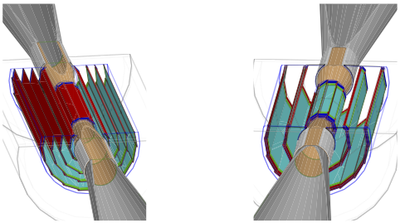
\includegraphics[width = 10 cm]{Pictures/vxd/ild_VXD.png}
     \caption{Overview of the two vertex detector options for the ILC. On the left, the VXD is made of five single sided layers, whereas the right option features three double-sided layers.}
     \label{fig:ild_vxd}
   \end{figure}

   \begin{table}[!tbh]
     \centering
     \begin{tabular}{K{0.7cm} K{1.1cm} K{1.4cm} K{1.4cm} K{1.4cm} K{1.4cm} K{1.4cm} K{1.4cm}}
      \hline
            & & \multicolumn{2}{c}{DBD VXD} &  \multicolumn{2}{c}{Conservative VXD} & \multicolumn{2}{c}{Ambitious VXD} \tabularnewline
      Layer & $R~(\rm{mm})$  & $\sigma_{\rm{sp}}~(\rm{\mu m})$ & $\sigma_{\rm{time}}~(\rm{\mu s})$ & $\sigma_{\rm{sp}}~(\rm{\mu m})$ & $\sigma_{\rm{time}}~(\rm{\mu s})$ & $\sigma_{\rm{sp}}~(\rm{\mu m})$ & $\sigma_{\rm{time}}~(\rm{\mu s})$ \tabularnewline 
      \hline
      \hline
      L1 & $16$ & $3$ & $50$ & $4$ & $4$ & $3$ & $1$ \tabularnewline
      L2 & $18$ & $6$ & $100$ & $4$ & $4$ & $3$ & $1$ \tabularnewline
      \hline
      L3 & $37$ & $4$ & $100$ & $4$ & $8$ & $3$ & $2$ \tabularnewline
      L4 & $39$ & $4$ & $100$ & $4$ & $8$ & $3$ & $2$ \tabularnewline
      \hline
      L5 & $58$ & $4$ & $100$ & $4$ & $8$ & $3$ & $2$ \tabularnewline
      L6 & $60$ & $4$ & $100$ & $4$ & $8$ & $3$ & $2$ \tabularnewline
      \hline
     \end{tabular}
     \caption{Possible performances for the three double-sided layers vertex detector. $R$ is the radius position of the considered layer, $\sigma_{\rm{sp}}$ the spatial resolution and $\sigma_{\rm{time}}$ the integration time~\cite{Yorgos}. }
     \label{tab:ild_vxd}
   \end{table}

   Another aspect not discussed yet is the radiation tolerance of the detector, which is directly related to the beam background.
   The first layer is the most affected by the background and it should have a high radiation tolerance. 
   The required radiation tolerance is about $1~\rm{kGy}$ for the total ionising dose and a fluence of $10^{11}\rm{n}_{\rm{eq}}\rm{.cm}^{-2}$~\cite{Behnke2013}.

   The efficiency of the \gls{VXD} has also to be excellent in order to maximise the tracking performance.
   The efficiency is defined here as the ratio of detected particles over all the particles crossing the detector.
   If one layer of the vertex detector misses a hit, the track reconstruction will be less accurate 
   
   To summarise, the expected parameters for the \gls{ILC} are: 
   \begin{itemize}
     \item An excellent impact parameter resolution: $a \sim 5~\rm{\mu m}$ and $b \sim 10~\rm{\mu m}$,
     \item a material budget not exceeding $0.1~\%~\rm{X_0}$ per layer for the single-sided option ($0.16~\%~\rm{X_0}$ for the double one),
     \item radius of the first layer $\sim~15/16~\rm{mm}$,
     \item an occupancy below the percent level.
   \end{itemize}

   The currently considered technologies are presented below. 
    
   \subsubsection{FPCCD}
   
     The \gls{FPCCD}~\cite{CalanchaParedes} is based on \gls{CCD} processes.
     The sensor is using small pixels size ($\sim 5~\rm{\mu m}$) to provide a sub-micron spatial resolution and an excellent capability to separate two nearby tracks.
     Its thickness is $50~\rm{\mu m}$ and the epitaxial layer ($15~\rm{\mu m}$ thick) is completely depleted to limit the charge spreading around pixels and to reduce the number of hits per pixel.
     However, the \gls{CCD} architecture provides slow readout and the matrix will be read between consecutive bunch trains, helping to reduce the power consumption and avoiding beam induced RF noise.
     Due to the radiation tolerance, the \gls{FPCCD} is operated at $-40 \degres \rm{C}$.

   \subsubsection{DEPFET}
    
    The \gls{DEPFET}~\cite{Richter2003} is an \gls{APS} in which field effect transistors are incorporated into each pixel.
    The single point resolution is $\sim 3~\rm{\mu m}$ for pixels with a size of $20~\rm{\mu m}$.
    The silicon itself is used as the sensitive part but also as a mechanical structure, minimising the support and services.
    The sensor is completely depleted of free charge carriers thanks to a voltage applied all along the sensor's thickness.
    The rolling-shutter approach is used for reading each row and the column readout is done by two auxiliary \glspl{ASIC}.
    As this technology is not made from standard industrial processes such as \gls{CCD} or \gls{CMOS} sensors, the cost of fabrication is higher than the two other technologies.

    \gls{DEPFET} technology has been chosen  to build the vertex detector of the BELLE-II experiment~\cite{depfetBelleII}.

   \subsubsection{CMOS}

   Different options for \gls{CMOS} pixel sensors are studied, such as 3D integrated \gls{CMOS}, but due to the context of this thesis, the work will focus on planar technologies developed by the \gls{IPHC} of Strasbourg: the \gls{MIMOSA} architecture. 
   This technology is described in section~\ref{sec:CMOS}.
  % The STAR experiment at RHIC is the first one to get an entire vertex detector made of ULTIMATE-MIMOSA28 CMOS sensors.
   %One of the technology developed is described in section~\ref{sec:CMOS}.

   For all technologies, the power consumption of the sensors is one of the key point in the \gls{VXD} design.
   The higher the power consumption, the more complex the cooling system is and higher the material budget in the sensitive area is.
   As it was shown in figure~\ref{fig:bunches} of chapter~\ref{chap:ILC}, the bunch train will last less than $1~\rm{ms}$ for a dead time of $199~\rm{ms}$.
   Two possibilities are envisaged to benefit from beam structure.
   For the first one, the hit information is stored using a time stamp during the bunch crossings and the data are read out after the last collision.
   This method might be used by the \gls{FPCCD} technology because of the slow integration time of the \gls{CCD} or with the \gls{MIMOSA}-26 sensors.
   Another solution is to use a \textit{power-pulsing} method.
   Right after the last collision, the sensors are switched off or the power consumption is reduced as mush as possible.
   Before the first collision, the sensors are switched on again.
   This pulsing method is investigated by different collaborations and is introduced for a single \gls{MIMOSA}-26 sensors in section~\ref{sec:perspectives}. 
   
   
  \section{PLUME}

  The \acrfull{PLUME} project aims to produce double-sided ladder prototypes driven by \gls{ILC} requirements~\cite{PLUME}.
  Three labs in Europe are involved: the \gls{PICSEL} group at the \gls{IPHC} in Strasbourg, the University of Bristol and \gls{DESY} in Hamburg.
  The collaboration is studying the feasibility to build such elements of vertex detector using \gls{MAPS} thinned down to $50~\rm{\mu m}$ and is exploring the benefits of this design.
  Strasbourg is developing and mounting the sensors on the modules, to take care of the readout and the \gls{DAQ}, and to provide a cooling system.
  The mechanical design, stability measurements and assembly procedure of the ladders are done by the University of Bristol, while \gls{DESY} has studied the ladder mock-up, performed power-pulsing tests and is now characterising and validating the modules in the lab.
  In 2016, DESY has provided the opportunity to test the ladder in real conditions thanks to the test beam facility and the possibility to use the \gls{DAQ} software developed at DESY: EUDAQ~\cite{EUDAQ}.

    \subsection{Design and goals}

    \begin{figure}[!tbh]
      \centering
      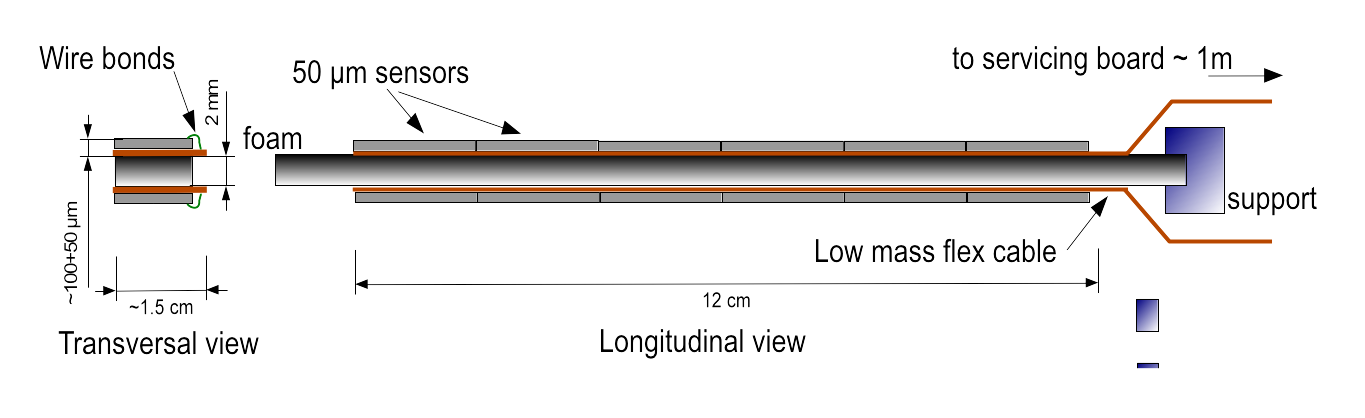
\includegraphics[width = 15 cm]{Pictures/vxd/plume_finalGoal.png}
      \caption{Side view (transversal and longitudinal) of the PLUME mechanical structure.}
      \label{fig:PLUME}
    \end{figure}

    Figure~\ref{fig:PLUME} illustrates the design of a PLUME ladder.
    The ladder structure is defined by the sensors arrangement on the mechanical support (positioned next to each other).
    In this design, the stiffener is a $2~\rm{mm}$ thick \gls{SiC} foam which has a density varying between $8~\%$ and $4~\%$ (depending on the ladder version) and could be reduced to only $2$ or $3~\%$.
    The choice of this foam results in a good compromise between the stiffness and the thickness compared to other materials~\cite{LectureJoel}.
    Figure~\ref{fig:YoungModulus} represents the Young Modulus as a function of the radiation length for different materials.
    The structure of the \gls{SiC} foam is shown in figure~\ref{fig:SiC}.
    It is macroscopically uniform and has the advantage of being easily machinable.
    Nevertheless, it has a low thermal conductivity ($50~\rm{W.m^{-1}.K^{-1}}$) and cannot be used to dissipate the heat trough contact.
    On each side of the stiffener, a low mass flex-cable is glued, which is used to connect the sensors for powering and managing them.
    It is made of copper traces coated in Kapton, but new prototypes using aluminum traces are developed and currently tested in order to reduce the material budget.
    %It is made of copper traces (prototype before 2011) or aluminum traces (new prototypes) coated in Kapton. 
    The ladder embeds twelve sensors, six on each face, that are glued and wire-bonded to the flex cable.
    On each flex-cable, a \gls{ZIF} connector is used for linking the modules to two external servicing boards, using a jumper cable.
    %On one edge of the flex-cable, a single \gls{ZIF} connector is used to link a module to the external board servicing, via a jumper cable.
    For the moment, the design is dedicated to the \gls{MIMOSA}-26 sensors thinned down to $50~\rm{\mu m}$ but it can be adapted to any kind of \gls{MAPS} sensors having the same thickness. 
    The main issues for the integration of \gls{MIMOSA}-26 comes from power pulsing ability, as well as the power dissipation of these sensors.
    This issues will be discussed in the next section (see~\ref{sec:prototypes}).
    %Although the \gls{MIMOSA}-26 has a spatial resolution better than $3~\rm{\mu m}$ (see section~\ref{subsec:Mi26}), the integration time is not suited for the bunch train structures of the \gls{ILC}.

    \begin{figure}[!tbh]
      \centering
      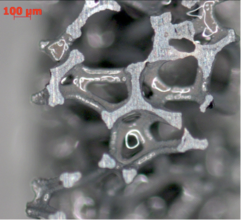
\includegraphics[width=0.3\textwidth]{Pictures/vxd/foam2.png}
      \caption{Microscopical view of the silicon carbide foam structure.}
      \label{fig:SiC}
    \end{figure}

    \begin{figure}[!tbh]
      \centering
      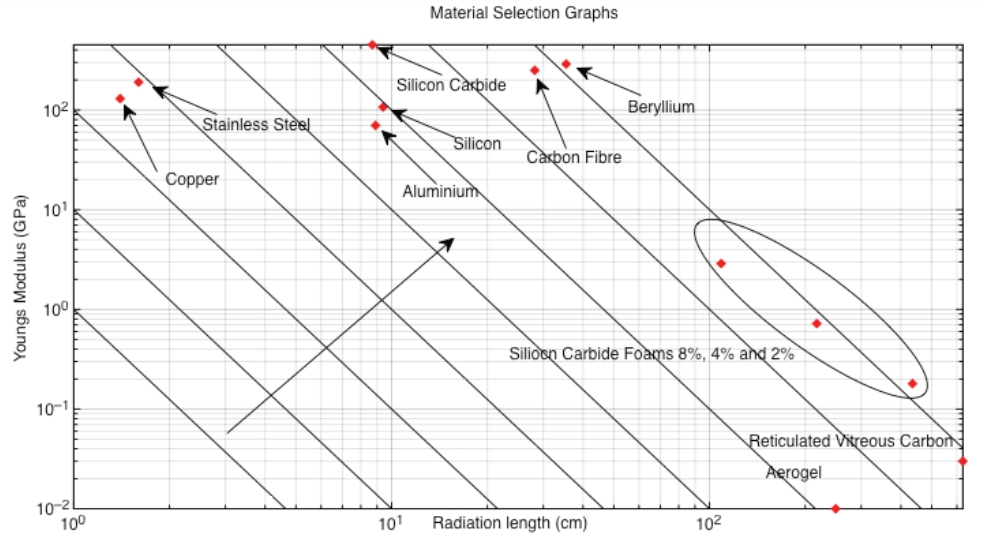
\includegraphics[width = \textwidth]{Pictures/vxd/youngModulus_vs_radiationLength-004.jpg}
      \caption{Graph of the Young modulus in GPa as a function of the radiation length in cm for different materials.}
      \label{fig:YoungModulus}
    \end{figure}

    The aims of the collaboration are to build ladders with a material budget better than $0.35~\%~\rm{X_0}$ for a spatial resolution better than $3~\rm{\mu m}$, and to evaluate the benefits of a double-sided measurement.

    \subsection{Prototypes}
    \label{sec:prototypes}

    Since 2009, the collaboration is studying the design, the production, the impact of the mechanical structure on the ladder's performances, but also how to power and control the sensors together.
    The first ladder prototype, called version-0 (V-0) was developed and tested in 2009.
    The purpose of this prototype was to settle the fabrication and the test beam procedures, without trying to reach the desired material budget goal.
    Two MIMOSA-20 analog output sensors were mounted on each side of a stiffener, providing a $1 \times 4~\rm{cm}^2$ sensitive area.
    The prototype was tested in $120~\rm{GeV}$ pion beam at the CERN-SPS and the results have demonstrated the benefits of the double-sided measurement on the spatial resolution, which is improved by a factor of about $1/\sqrt{2}$~\cite{Nomerotski}.

    \begin{figure}[!tbh]
      \centering
      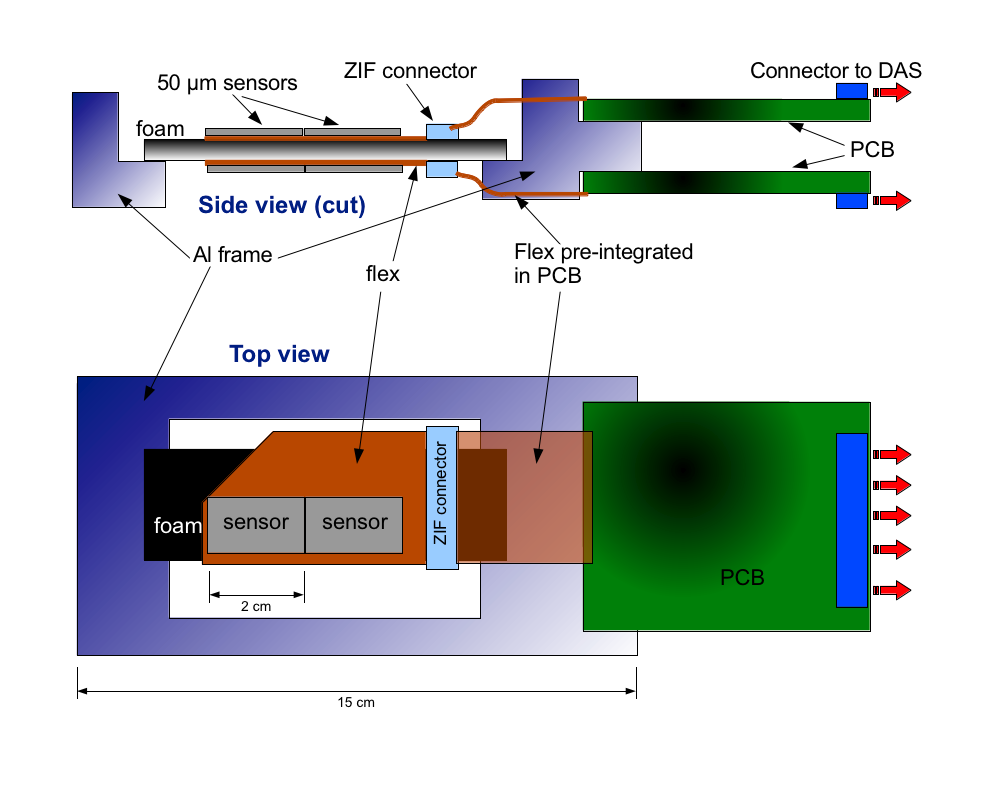
\includegraphics[width = \textwidth]{Pictures/vxd/bos_ladder_v1_PLUME0.png}
      \caption{Side and top view of the first PLUME prototype built in 2009.}
    \end{figure}

    Then in 2010, a second prototype featuring the desired sensitive surface, called version-1 (V-1), was developed.
    Each module of the ladder was made of Kapton flex-cable with a thickness of $0.14~\rm{mm}$, using copper traces.
    These modules are called \gls{OKF}, where Optiprint is the vendor of these flex-cables.
    It is the first version to embed six \gls{MIMOSA}-26 binary output sensors working simultaneously on each side of the stiffener.
    The material budget is estimated to be $0.65~\% ~\rm{of}~\rm{X_0}$ in the sensor's sensitive area. 
    The aim of this prototype was to validate the operation of multiple sensors in a chain.
    Two ladders were tested in real conditions.
    The first one was tested with $120~\rm{GeV}$ pions at CERN-SPS in 2011, while the second ladder was tested in April 2016 with up to $5~\rm{GeV}$ positrons at DESY in Hamburg. 
    The DESY test beam results are presented in chapter~\ref{chap:X0}, while a specific study of the sensors' deformation observed at CERN in 2011 is discussed in chapter~\ref{chap:deformation}.

    \begin{figure}[!tbh]
      \centering
      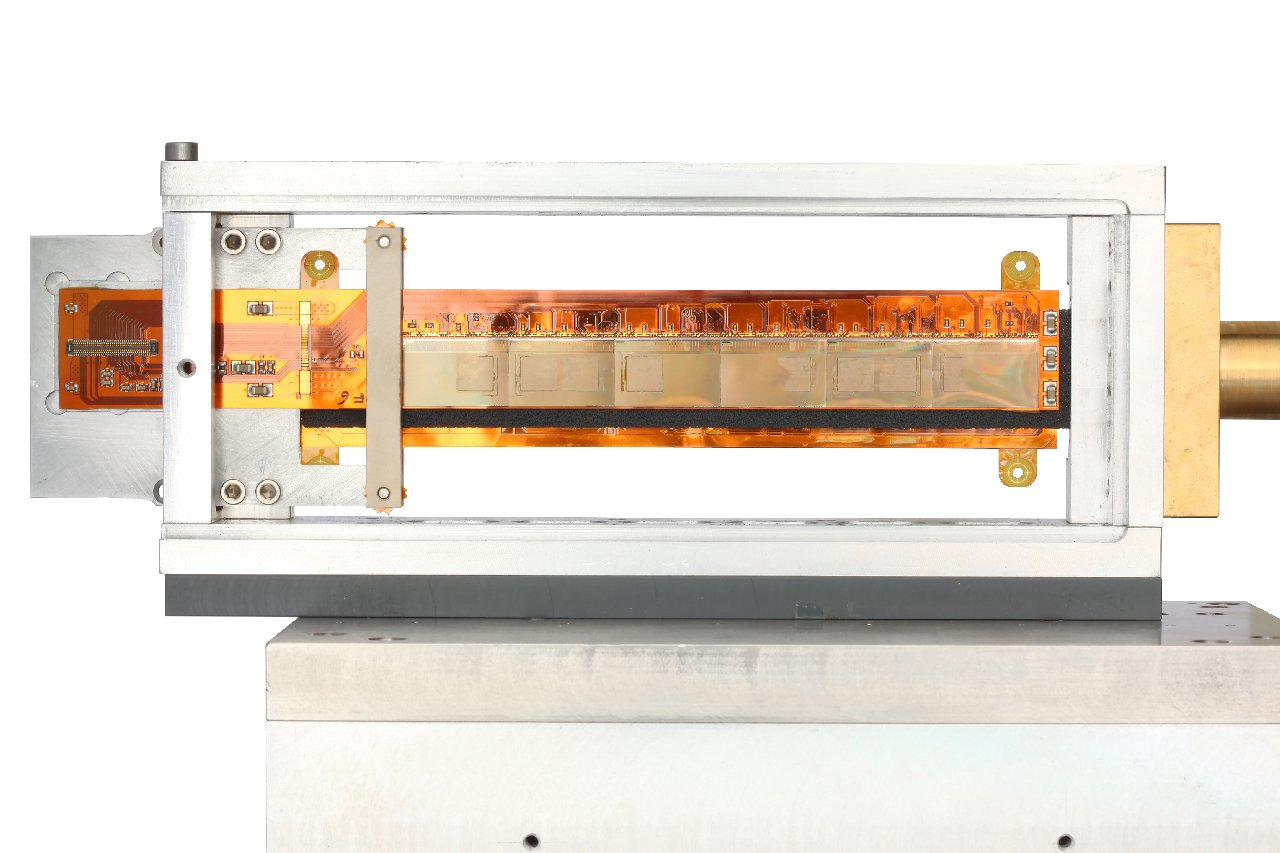
\includegraphics[width = 12 cm]{Pictures/vxd/plume_ladder2010_frontView}
      \caption{Front view of the ladder version-1 made in 2010 in its holding box. On the left, there is the connector to the output board servicing, on the right a connection to blow air on the module. As this version was not made with a mirrored design, the flexible cables are not entirely overlapping and the SiC foam can be seen (in black here).}
    \end{figure}

    At the beginning of 2016, the third prototype versions were mounted but have not yet been completely tested.
    In fact, this new version is divided into two sub-versions: one using copper traces and the other one aluminum traces.
    Nevertheless, both sub-versions have a new design featuring reduced traces thickness to have a narrower flex-cable ($18~\rm{mm}$ width) adjusted to the sensors width in order to minimise the dead areas.
    The flex-design has slightly changed to have a mirrored geometry (figure~\ref{fig:AM01}) and a straight geometry in order to minimize the dead area too and have a better alignment solution.
    The stiffener is made of a lower density \gls{SiC} foam reducing the global material budget. 

    \begin{figure}[!tbh]
      \centering
      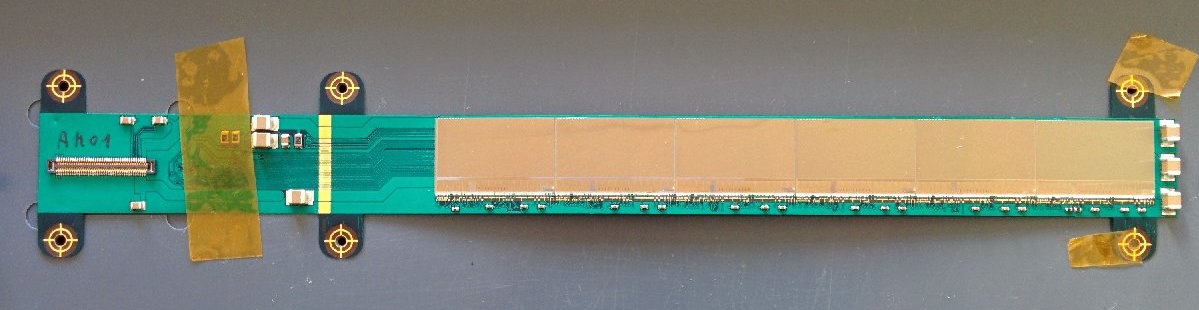
\includegraphics[width = 12cm]{Pictures/vxd/AM01.jpg}
      \caption{Picture of the first mirrored module made with aluminum traces. The cable width is adjusted to the size of the sensor.}
      \label{fig:AM01}
    \end{figure}
    
    Table~\ref{tab:X0} summarises the material budget reached by the different prototypes.

    \begin{table}[!tbh]
      \begin{center}
        \begin{tabular}{c c c c c c c}
        \hline %----------------------------
        \multirow{2}*{Layer}  & \multicolumn{3}{ c }{budget (\% X$_0$)}  \tabularnewline
                              &  V-0 & V-1 & Goal \tabularnewline
        \hline %----------------------------
        \hline %----------------------------
        Sensor (x2)           & 0.106 & 0.106 & 0.106 \tabularnewline
        Flex-cable (x2)       & 1.048 & 0.300 & 0.068 \tabularnewline
        Glue (x4)             & 0.04  & 0.04  & 0.04  \tabularnewline
        Passive components    & 0     & 0.033 & 0.033 \tabularnewline
        Stiffener (foam)      & 0.764 & 0.175 & 0.087 \tabularnewline
        \hline %----------------------------
        \textbf{Total}        & 1.926 & 0.654 & 0.334 \tabularnewline
        \hline %----------------------------
        \end{tabular}
        \caption{Estimation of the material budget for the different prototypes of the PLUME ladder.}
        \label{tab:X0}
      \end{center}
    \end{table}

    \subsection{Perspectives}
    \label{sec:perspectives}

    Although the collaboration has shown their expertise in building light mechanical structures, more tests and optimisations have to be done.
    MIMOSA-26 sensors are not designed to match the \gls{ILC} specifications. 
    Since a bunch train at the \gls{ILC} last only $0.95~\rm{ms}$ and the integration time of this sensor is $115.2~\rm{\mu s}$, a new CPS with a faster integration time has to be integrated.
    Another problem of the MIMOSA-26 sensors is that they are not suited for power-pulsing scheme. 
    Remember that the principle of the power pulsing is to reduce the consumption of the sensor during the $200~\rm{ms}$ dead time. 
    Nevertheless, a power-pulsing study on a single Mi-26 sensor has been done and the results have shown that the nominal supply voltage of the MIMOSA-26 can be lowered from $3.3~\rm{V}$ to $1.85~\rm{V}$ without losing the sensor's registers. 
    The fake hit rate measured was close to the one obtained in  normal conditions after the sensor reaches a stable operation.
    Moreover, the power consumption was reduced by a factor of 6.3~\cite{Kuprash2013}. 

    A complete power-pulsing study of the whole ladder has to be done in the lab in order to make sure that the sensors are still behaving correctly.
    If the first results are promising, the power-pulsing will be tested under real conditions with a high magnetic field.
    The impact of the Lorentz forces due to the coupling of the power-pulsing and the magnetic field is going to be studied, especially if this structure will induce unwanted deformations or vibrations. 

    %The collaboration is considering to embed the sensors directly inside the multi-layer micro-cable~\cite{Baudot2012}.
    %The chips are glued on the first polyimide substrate layer, then the metal layer is deposited on top of it and the metal traces are directly connected to the chips pads.
    %Then an insulator is added to the module.
    %The advantages of this technique are, firstly, the direct connection of metal traces to the pads that avoid wire-bonding and can reduce, at the same time, the width of the module.
    %And secondly, this structure has the advantage to apply the mechanical stress on the polymer wrapping, thus reducing it on the sensor.

    A closer perspective for the collaboration is to integrate two ladders in the physics commissioning of the \gls{BEAST} experiment at KEK~\cite{Ye}.

  \section{Integration of CMOS sensors}
  \label{sec:CMOS}

  %Since the beginning of the 1990's, a new alternative to the \gls{CCD} was developed by the imaging industry: the \gls{APS}.
  %They have produced thanks to the \gls{CMOS} industrial process and are equipping nowadays the sensors of the camera.
  %They are called so because the pixel is made of a photodiode associated with an active amplifier.
  %They are called active pixel sensors because the pixel is made of a photodiode  and an active amplifier. 
  %This technology is well used in the industry and equipped most of the camera produced.

  The PICSEL group of the IPHC at Strasbourg is developing since 1999 CMOS sensors called MIMOSA for \textit{Minimum Ionizing MOS Active pixel sensor}. 
  They are semi-conducting pixel sensors based on the \gls{APS}, an alternative to the \gls{CCD} technology.
  The imaging industry developed this technology at the beginning of the 1990's, and it is used nowadays in commercial applications, like smartphone's cameras.
  One particularity of the sensors developed by Strasbourg is that the various functionalities, such the sensitive area and the electronic layer where the signal is processed, are made of the same material.
  This device is called then \acrfull{MAPS} and the different layers are:
  \begin{itemize}
    \item a substrate providing mechanical stability;
    \item an epitaxial layer which is the sensitive volume of the sensor;
    \item an electronic layer where the diodes collecting the charges and the micro-circuits processing the signal are located.
  \end{itemize}

  The motivation to use this technology or any other silicon sensor in particle physics is due to the minimum energy needed to create an electron/hole pair by a traversing particle.
  In silicon, this minimum energy is only $3.6~\rm{eV}$, while for a gaseous detector, it is close to $30~\rm{eV}$.

    \subsection{Charge creation and signal collection}   

    The \gls{CMOS} sensor can detect impinging particles thanks to their structure, but also to the interaction of particles with matter.
    When a charged particle is traversing a layer of matter, it loses energy via ionisations due to electromagnetic interactions with electrons and nuclei.
    Due to the size of a \gls{MAPS}, charged particle loses only a small fraction of its energy, and the spread of the energy loss can be described by a Landau distribution.
    A \gls{MIP} creates 80 electrons per microns inside the silicon.

    At the beginning, the microelectronic industry has insulated the transistors from the substrate using a high-resistivity layer, called the epitaxial layer.
    The development of \gls{CMOS} sensors was accelerated due to the properties offered by these semiconductors.
    
    %The different structure of the sensor has distinct doping.
    %The bulk is a P++ doped layer made with a moderate quality silicon.
    %The crystal structure has many defects leading to a high rate recombination of charge carriers.
    %Above the substrate, the epitaxial layer is P- doped and made of a good quality silicon.
    %The electron/hole pairs created in this layer do not recombine instantaneously like in a highly doped layer but they are thermally diffused. 
    
    The \gls{CMOS} sensors developed by the IPHC at Strasbourg are called monolithic \gls{MAPS} sensors because the different layers of the sensor are made in one block of the same material, but with different doping.
    The structure of the sensor is a highly doped P+ substrate made of a moderate quality silicon. 
    The crystal structure contains a lot of defects, hence the recombination rate of charge carriers is high.
    Above this bulk, a low-doping P- layer is grown.
    The silicon used is good quality, thus the charge carriers have less chance to recombine.
    This layer is the sensitive part of the sensor and is called the epitaxial layer. 
    On top of it, an N-well implant has the role of charge collection.
    The interface between the N-wells and the epitaxial layer forms a P-N junction called a collection diode.
    A depleted area is created by this junction, on which the charge carriers are attracted.
    Nevertheless, this P-N junction is only one part of the pixel.
    Next to the N-well implants sit  highly-doped P-wells used to reflect the charge carriers to the implants.
    The difference of doping between the bulk and the epitaxial layer is also used to reflect the charge carriers to the collection diode.

    The typical doping concentration are $10^{15}~\rm{at.cm}^{-3}$ for the epitaxial layer, $10^{19}~\rm{at.cm}^{-3}$ in the substrate and $10^{17}~\rm{at.cm}^{-3}$ for the other layers.
    The doping concentration defines the size of the depleted region.
    For these doping concentrations, only a small region around the P-N junction is depleted, while the epitaxial layer is mainly undepleted. 
    As no external voltage is applied to the sensor to increase the depleted region, the charge carriers created by crossing particles are thermally diffused from the epitaxial layer to the diode.
    Nevertheless, the different doping levels produce a built-in voltage defined as: 

    \begin{equation}
      V_b = \frac{kT}{q}ln\left( \frac{N_{p+}}{N_{p-}}\right)i.
    \end{equation}
    
    The built-in voltage depends on the Boltzmann constant $k$, the temperature $T$, the elementary charge $q$ and the different concentrations doping $N_{p\pm}$ of the interface.
    Due to the different doping levels, the electrons are restricted to diffuse inside the sensitive volume, to be then guided towards a collection diode.
    One effect of the thermal diffusion is that the average path of the electrons in the epitaxial layer is longer than the one they would have in a fully-depleted sensor.
    Hence, the probability of recombination between an electron and a hole increases.
    Also, the charges tend to spread more around neighboring n-well.
    Therefore, the charge collection efficiency is lower than the fully-depleted sensor.

    \begin{figure}[!tbh]
      \centering
      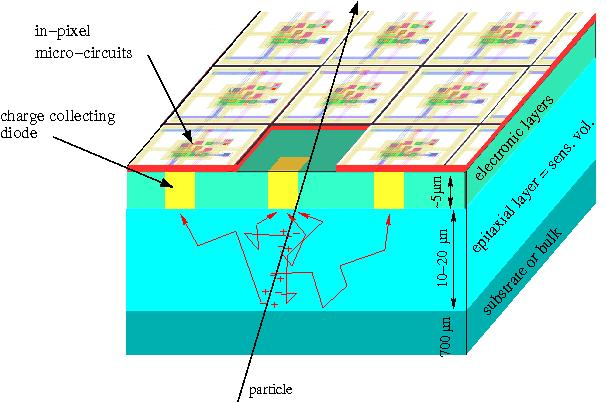
\includegraphics[width = 10cm]{Pictures/vxd/principeMapsMIP.jpg}
      \caption{Drawing of MAPS structure representing the different layers of the sensor and the path of charge carriers in the epitaxial layer.}
      \label{fig:principleMaps}
    \end{figure}

    \subsection{Advantages and disadvantages of the technology}

    \gls{CMOS} sensors have several interesting properties.
    First of all, the fabrication cost is lower than other pixel technologies due to the industrial processes used to build the sensors.
    Therefore, many prototypes and bigger matrices can be built, while benefiting from the industrial experience.
    The limit toward small pixels is fixed by the number of transistors embedded in a pixel.
    Smaller grid sizes with a pitch size of few microns are built by the imaging industry.
    
    Secondly, due to the size of the depleted area, the charge carriers tend to spread more over neighboring pixels.
    On the one hand, the signal collected per pixel is smaller, but on the other hand, the reconstruction of the hit position with a centre of gravity algorithm is improving the spatial resolution.
    To give an idea, a binary output sensor with a pitch of $18.4~\rm{\mu m}$ can achieve a spatial resolution better than $3~\rm{\mu m}$.
    Figure~\ref{fig:pitchVsSR} shows the evolution of the spatial resolution achieved for different pitch size for different \gls{MIMOSA} sensors.

    \begin{figure}[!tbh]
      \centering
      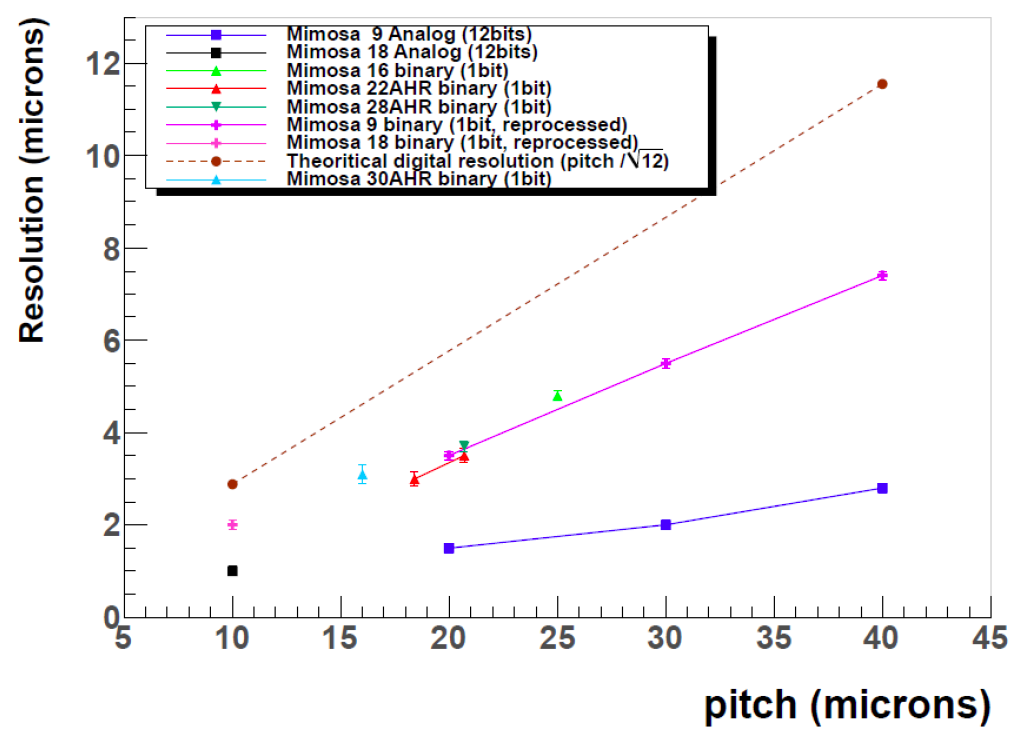
\includegraphics[width = 0.7\textwidth]{Pictures/vxd/resolution_pitch_10to40_withBinary.png}
      \caption{Evolution of the spatial resolution achieved for different pitch sizes and for different MIMOSA sensors.}
      \label{fig:pitchVsSR}
    \end{figure}

    Thirdly, the different doping of the different layers is responsible for the reflection of the charge carriers to the collection diodes.
    However, only the interface between two different doped regions is responsible for this reflection.
    Figure~\ref{fig:collectionEfield} shows the principle of the charge collection at the interface between the substrate and the epitaxial layer.
    The substrate can be thinned down to few microns leading to a sensor with a thickness of $50~\rm{\mu m}$, while keeping the possibility to manipulate them.
    In this way, the material budget can be reduced down to $0.053~\%~\rm{X_0}$.
    %The bulk is not entirely responsible for the charge carriers reflection, only the interface between the substrate and the epitaxial layer is mainly responsible for the reflection.
    %The substrate can be thinned down to few microns leading to a sensor with a thickness of 50 $\mu\text{m}$ while keeping the possibility to manipulate them.
    %The material budget can then be reduced to 0.053 \%.

    \begin{figure}[!tbh]
      \centering
      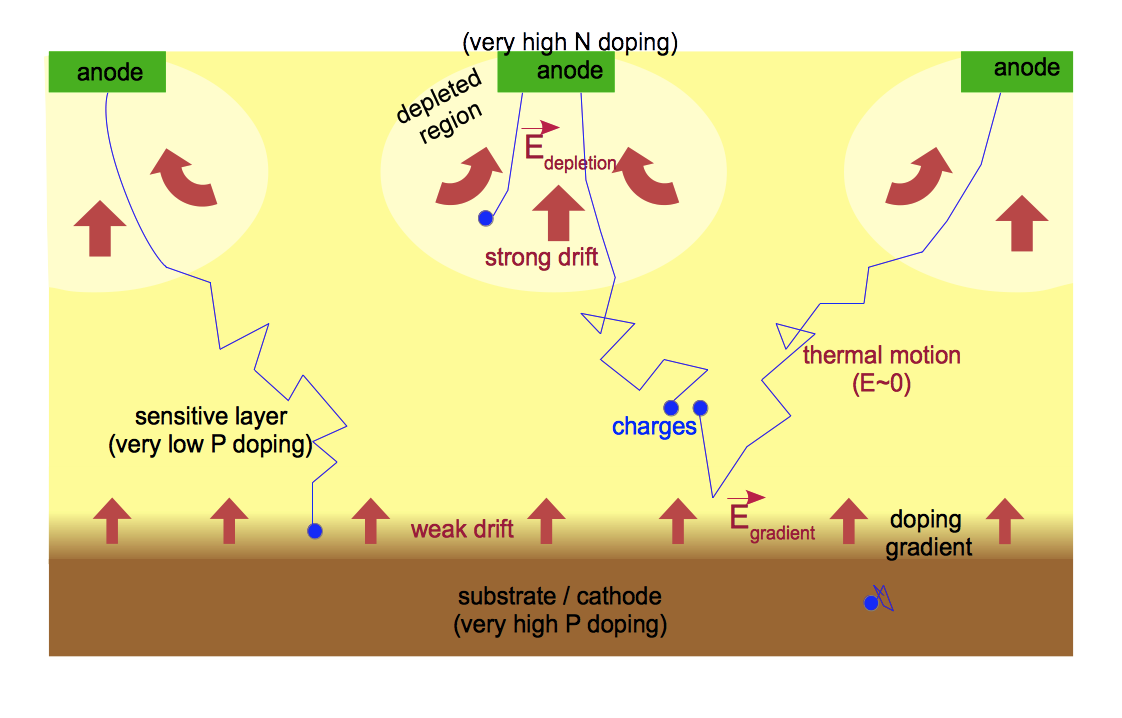
\includegraphics[width = \textwidth]{Pictures/vxd/collectionEfield.png}
      \caption{Principle of charge collection in a MAPS. The difference of doping between the substrate and the epitaxial layers create a reflection region.}
      \label{fig:collectionEfield}
    \end{figure}

    Nevertheless, the thickness of the epitaxial layer (usually between $10$ and $15~\rm{\mu m}$) and the small depleted region (in the order of $1$ to $5~\rm{\mu m}$) are responsible for a small charge collection.
    As a matter of fact, a \gls{MIP} is creating 80 electron/hole pairs per micron, so the number of charges collected by the diode is of the order of a thousand electrons.
    Hence, the signal created is only a few millivolts and low noise electronics have to be used for processing the signal.

    \gls{CMOS} sensors are sensitive to ionising and non-ionising radiations which degrade the sensor properties.
    The non-ionising radiation damages the crystal structure of the epitaxial layers, creating defects in the lattice.
    The recombination rate is increased and reduces the signal collected.
    To avoid this effect, two solutions are possible.
    The first one is to reduce the size of the pixels in order to decrease the path of the particles from the epitaxial layer to the collection diodes.
    Nevertheless, a smaller pitch size induces a slower readout and the cost to build such a sensor increases.
    The second solution is to increase the resistivity of the epitaxial layer to expand the depleted area.
    
    The ionising radiation is responsible for charge accumulation in oxides at the interface with silicon layers.
    The leakage current increases in the pixel and diode collection.
    The ionising dose increases the noise, whereas the non-ionising fluence decreases the signal.
    %To reduce the leakage current, smaller diodes can be used to reduce the impact of the leakage current but, as was explained before, the cost of fabrication increases.
    
    \subsection{Signal processing}

    If no charge is collected by the pixel, the voltage at the equivalent capacitor of the diode is growing because of the leakage current inherent in the junction.
    The pixel reading can be done in two different ways, depending on the method used to minimise the leakage current effect.
    Currently, two pixel architectures are used to compensate the diode's leakage current: the \textit{3 Transistors pixel design}, mainly used in imaging, and the \textit{self-biased pixel design}.
    The circuit diagram which is shown in figure~\ref{fig:elecArch} represents the two methods to design pixels.
    
    \begin{figure}[!tbh]
      \centering
      \begin{subfigure}[t]{0.45\textwidth}
          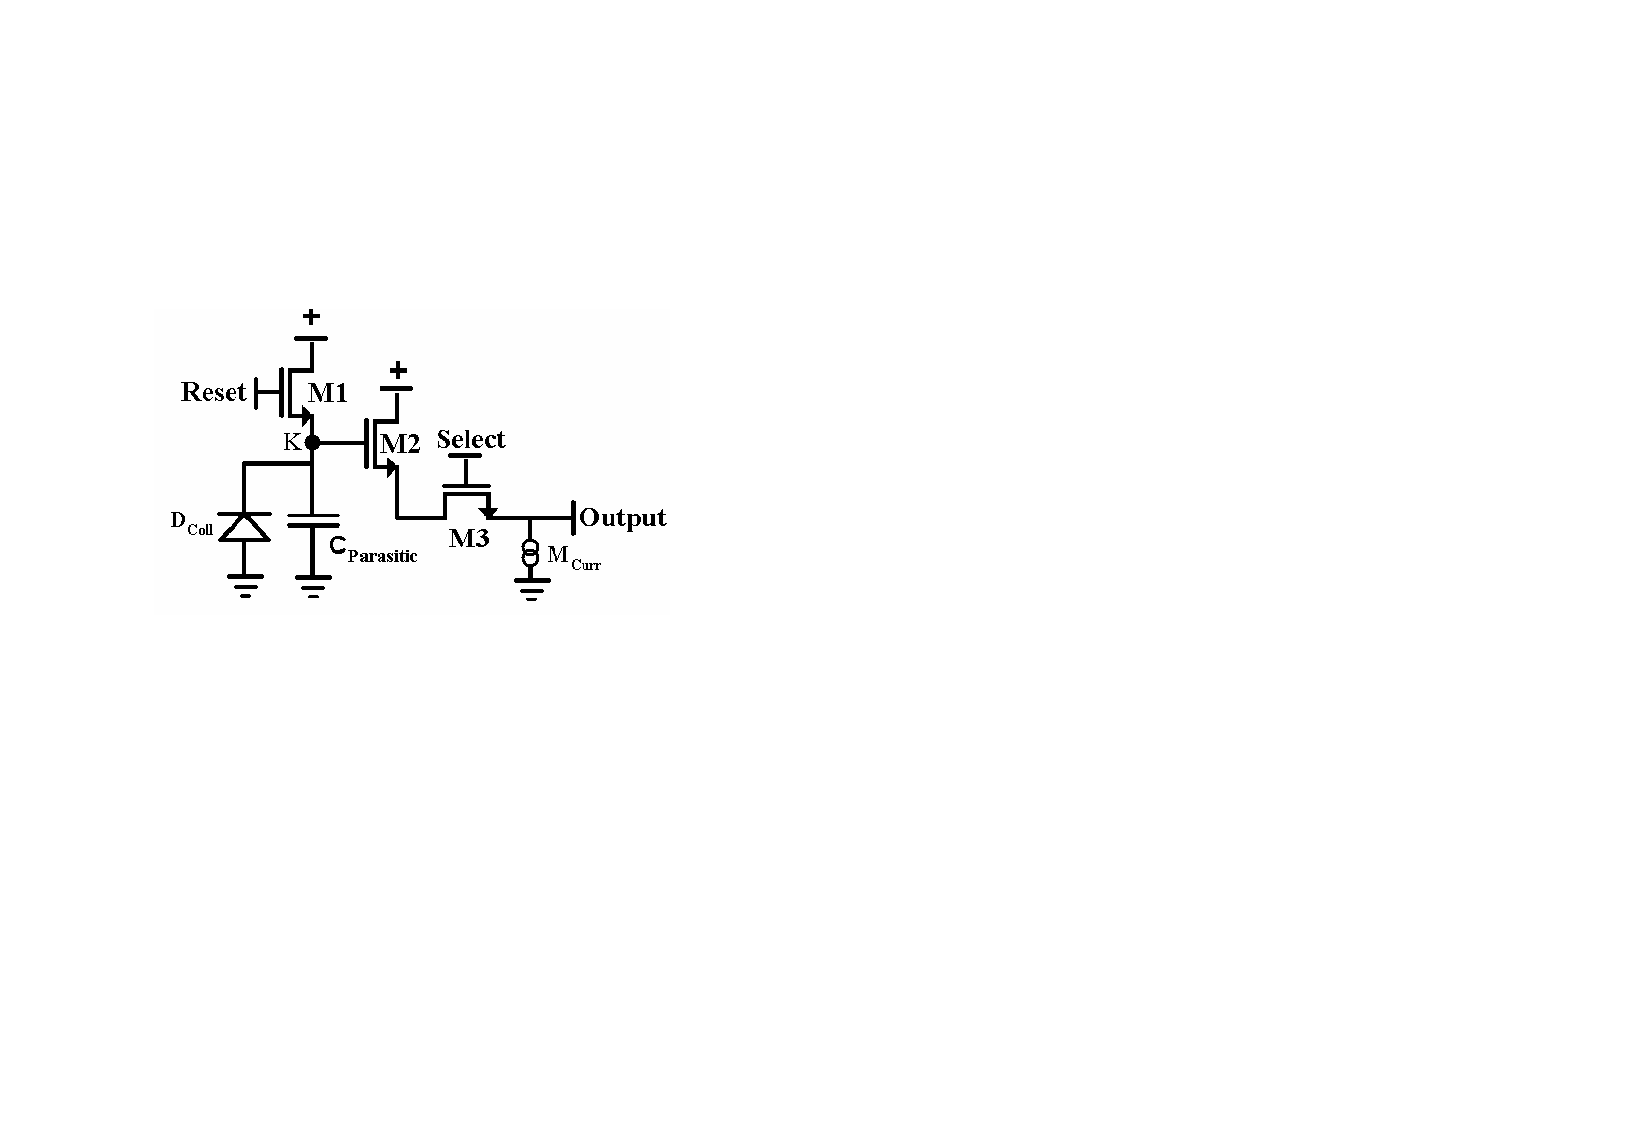
\includegraphics[width=\textwidth]{Pictures/vxd/3T_architecture.pdf}
          \caption{Three transistors (3T) pixel design.}
          \label{fig:3T}
      \end{subfigure}
      ~%\quad
       %add desired spacing between images, e. g. ~, \quad, \qquad, \hfill etc. 
        %(or a blank line to force the subfigure onto a new line)
      \begin{subfigure}[t]{0.45\textwidth}
          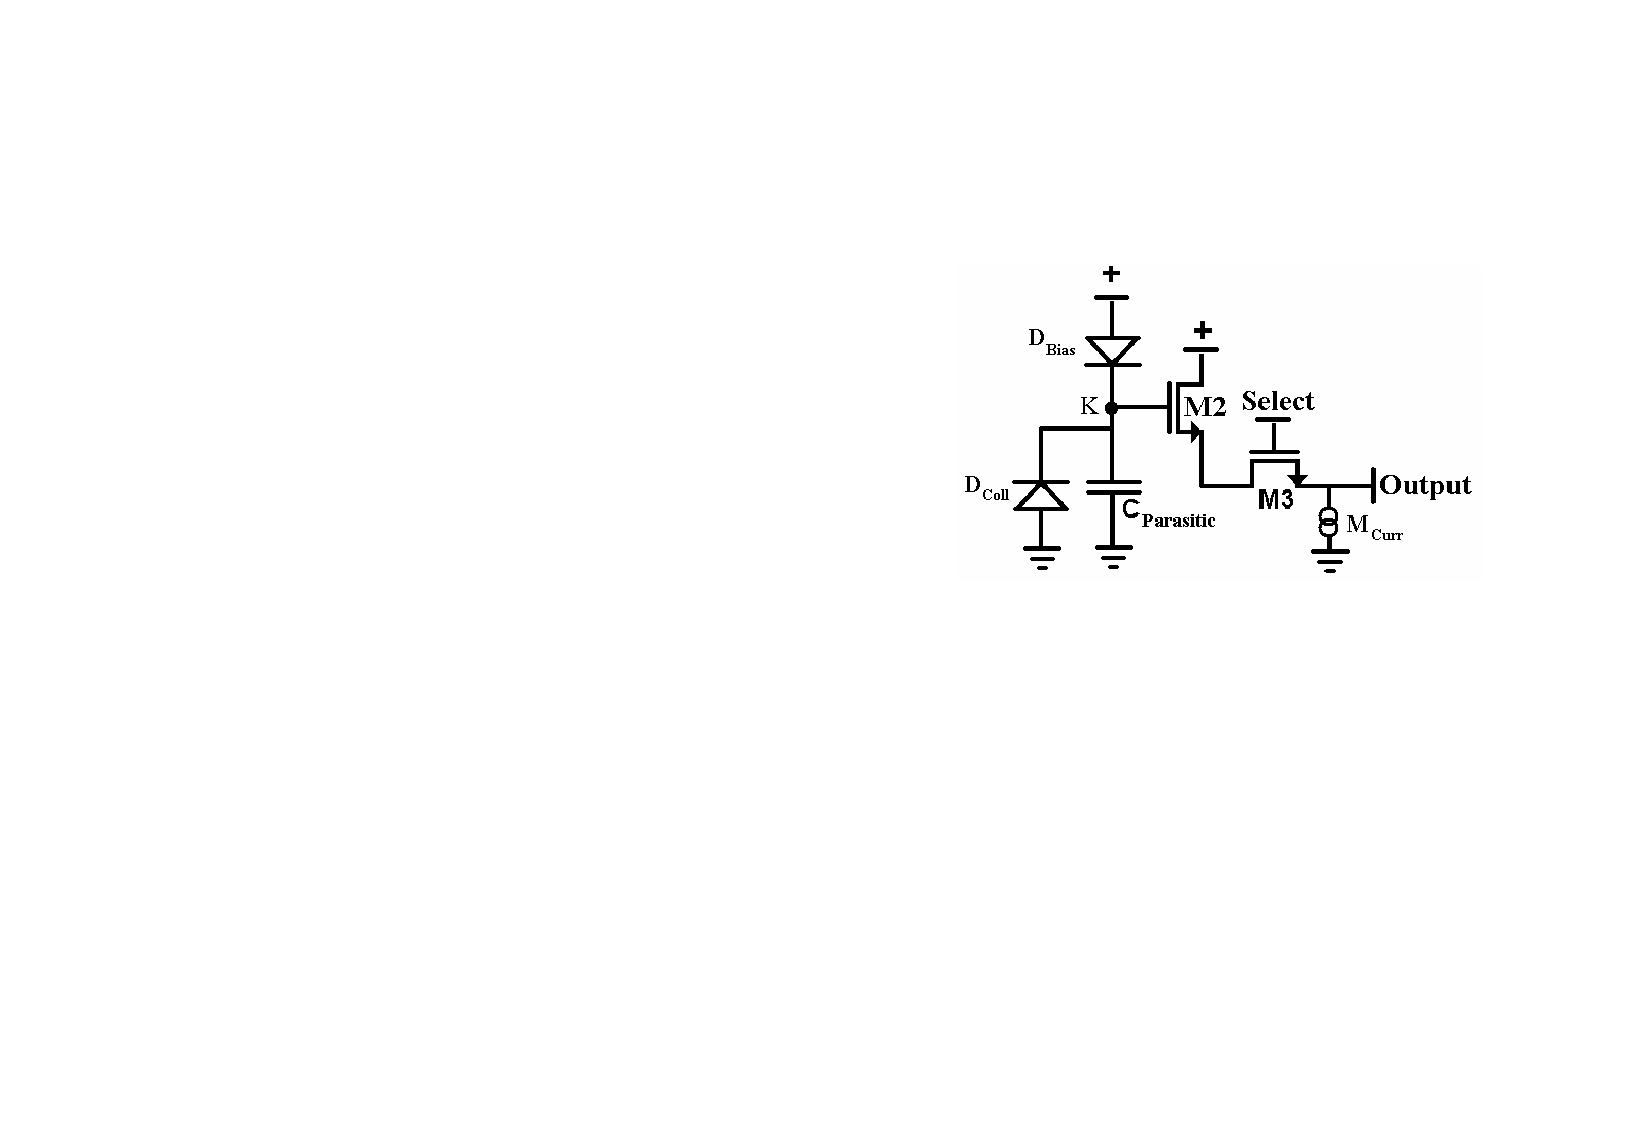
\includegraphics[width=0.95\textwidth]{Pictures/vxd/self-biased_architecture.pdf}
          \caption{Self-biased pixel design.}
          \label{fig:selfBiased}
      \end{subfigure}
      \caption{Two different architectures of pixel.}
      \label{fig:elecArch}
    \end{figure}    

    The first one, presented in figure~\ref{fig:3T}, consists of reinitialising the collection diode's voltage to a reference voltage thanks to a \textit{reset} transistor, denoted M1 on the diagram.
    This method works in two steps. 
    Firstly, the M1 transistor is closed and the charge of the equivalent capacitor $C_d$ associated to the junction P-N, represented by a diode on the diagram, is slowly decreasing because of the diode's leakage current. 
    During this phase, the pixel is sensitive and is read.
    After a time interval equivalent to the integration time of the sensor, the transistor M1 is opened to recharge $C_d$ to its initial voltage.
    During this time, the pixel is not sensitive.
    While M1 is used for the reset, M2 is used as a pre-amplifier of the signal created by the diode and M3 link-up the voltage to the output of the circuit.
    Although this compensation method is fast, it generates a dead time for detection between two readings.
    
    Figure~\ref{fig:selfBiased} depicts the \textit{self-biased pixel design} method~\cite{Deveaux2009}.
    It is using a P-N junction (symbolised here by a diode mounted on the other side) coupled to the N-well implant to absorb the leakage current.
    The inverted diode is continuously compensating the diode's leakage current, thus the dead time vanishes.
    %Using a forward p-n junction has the advantage to avoid any dead-time because the diode's leakage current is continuously compensated by the second diode.
    While no particle is crossing the sensor, an equilibrium appears between the leakage and recharge current.
    A particle going through the sensor disrupts this equilibrium.
    The charge collected by the pixel leads to a discharge of the diode's capacitor $C_d$, followed by a recharge of this capacitor thanks to the second diode to reach the equilibrium again.
    %When a particle is crossing the sensor, the charges are collected by the pixel, leading to a discharge of the diode's capacitor $C_d$, which is followed by a recharge to reach again the equilibrium.
    Nevertheless, if the recharge procedure is too fast compared to the integration time, the physics signal is masked and the passage of the particle is never notified.
    %Nevertheless, the recharge procedure should be slower than the integration time to be able to detect physics signal during detection.
    %Indeed, when the recharge is too fast, the physics signal is masked and the passage of particle will never be notified.
    Even if the time interval to recharge the capacitor $C_d$ is set properly, an important charge collection per pixel could disturb the recharge phase and the pixel will reach a stable level again only after a long time interval of the order of $10~\rm{ms}$.

    \subsubsection{Integration time and readout}

    For a non-depleted epitaxial layer, the charge carriers are mostly thermally diffused to the collection diodes.
    The time to collect these charges in a pixel is $\sim 100~\rm{ns}$, setting a maximal limit to read the signal.
    This integration time is not reachable due to other factors, like the pixel occupancy or the time needed to obtain the information of all the pixels.
    Also, a compromise to reach fast integration times has to be made.
    The faster the sensor, the more important the power consumption of the electronics becomes.
    Moreover, to reduce the integration time, a solution exists in increasing the size of the pixels.
    In consequence, the pointing resolution of the device is impacted.
    For the case of the \gls{ILC}, the integration time is dictated by the pixel occupancy that should not be bigger than a percent, to stay in the using sensor's range and to be able to use the pattern recognition for tracking.

    The first sensors were developed using an analog output.
    With this approach, the pixels were addressed sequentially and their output was multiplexed in one bus line.
    The advantage of such a method is that the discrimination can be adjusted offline for each pixel, thus compensating for a nonuniform response.
    Nevertheless, the integration time is dependent on the operational frequency of the bus (usually $50~\rm{MHz}$) and the number of pixels contained in a matrix.
    For a sensor having millions of pixels, the integration time is then of the order of a millisecond.
    An analog output is then too slow for \gls{ILC} purposes. 
    
    \begin{figure}[!tbh]
      \centering
      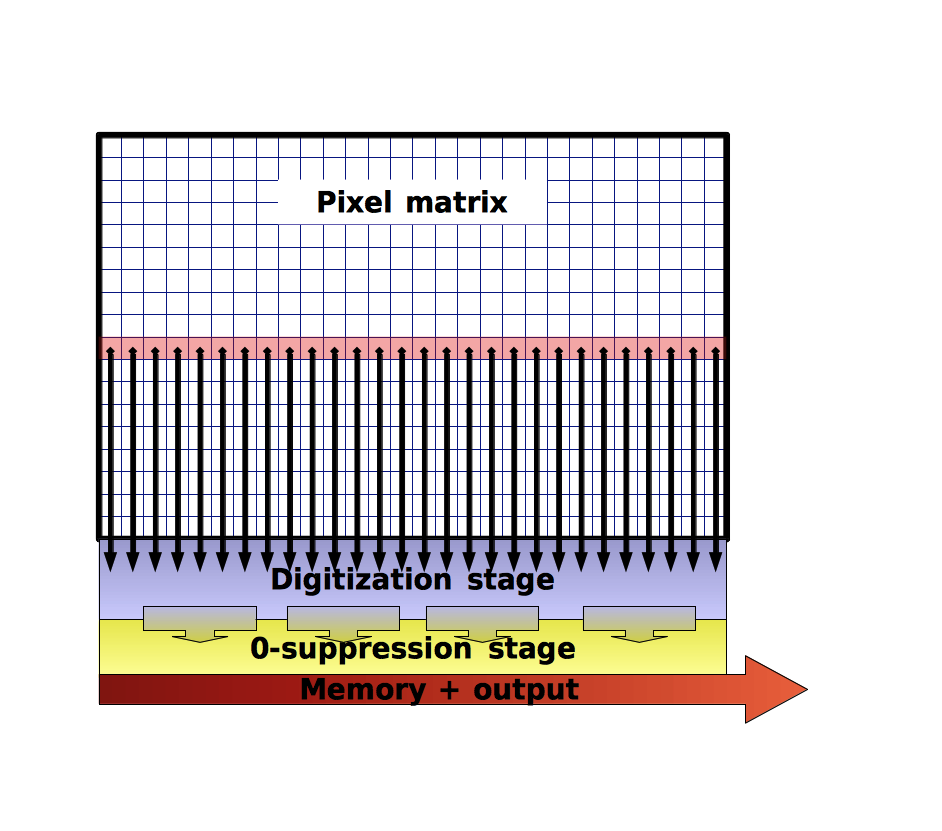
\includegraphics[width = 0.8\textwidth]{Pictures/vxd/parallelColumnPrinciple_2bis.png}
      \caption{Schematic operation of the parallel column readout.}
      \label{fig:rollShut}
    \end{figure}
    
    To overcome this problem, an approach is to group the pixels in columns and to read them in parallel.
    Figure~\ref{fig:rollShut} depicts the principle of this method called \textit{column parallel readout} or \textit{rolling-shutter}.
    Instead of having one bus line for the whole matrix, each column has its own bus and a data sparsification logic is integrated on the periphery of the sensor.
    One row is read out in between $100~\rm{ns}$ and $200~\rm{ns}$, independently of the number of pixels contained in it.
    As a consequence, a matrix containing thousands of rows has an integration time of $\mathcal{O}(100~\rm{\mu s})$.
    Moreover, to improve the integration time an output memory is duplicated at the periphery of the sensor.
    Hence, when one line is read, the precedent one is processed by the micro-circuits at the end of each bus line of each column.
    To minimise the data bandwidth, only the pixels above certain thresholds are read thanks to discriminators coupling to a zero suppression logic, called \gls{SUZE}~\cite{Himmi}.
    In this way, only the address of the first pixel hit in a row and the number of the adjacent fired ones are stored.
    This memory is duplicated to be able to process one row, while the previous one is read out by the outside world.
    In order to increase the readout speed, two techniques are conceivable~\cite{Winter:2009zz}.
    The first one provides elongated pixels in the vertical direction in order to reduce the number of rows, thus degrading the spatial resolution in the same direction.
    The second one consists of dividing the columns into two distinct parts, which have their dedicated output.

    \begin{figure}[!tbh]
      \centering
      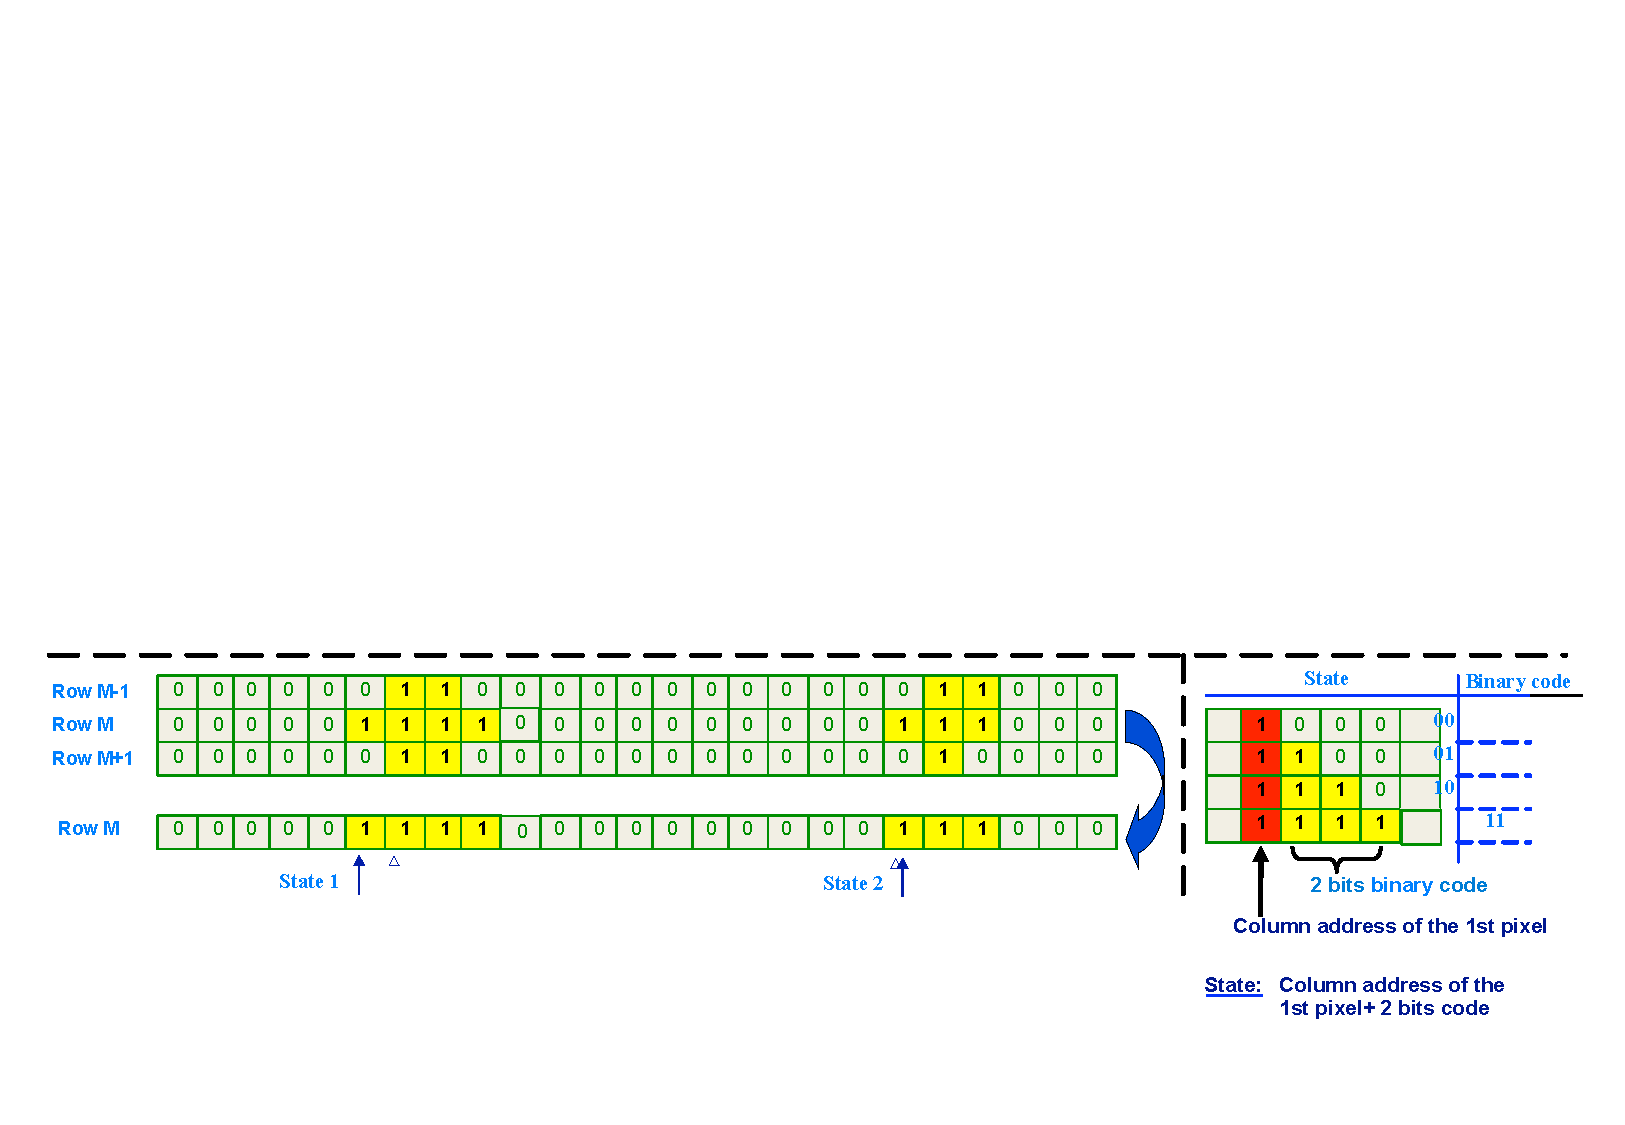
\includegraphics[width=\textwidth]{Pictures/vxd/suze_hit.pdf}
      \caption{Principle of the zero suppression logic. }
      \label{fig:SUZE}
    \end{figure}

    \subsubsection{Noise}

    An important figure of merit is the effective noise equivalent for one pixel.
    Many factors are driving this noise value and the different kind of noises are divided into two categories: the \gls{FPN} and the \gls{TN}.
    The nonuniform response of the pixels in a sub-array is responsible for the \gls{FPN} and is regarded as an offset between the pixel pedestals, which is subtracted from the pixel response to reduce the impact of this noise.
    The \gls{TN} has different origins, as the shot noise, the pink noise or the thermal noise.
    The different operational phases to read the signal are contributing to the noise.
    
    One contribution to the \gls{TN} appears in the \textit{3T pixel design} only during the reset phase.
    This noise arises when the transistor is open restoring the charge of the capacitor associated with the collection diode.
    It is dependent on the temperature and the diode's capacitance.
    
    The second one is the noise during integration and is caused by statistical fluctuations of the leakage current (shot noise).
    The faster the integration time, the smaller the shot noise contribution becomes.
    
    Finally, the third one arises from the readout, while the column switch and the source follower capacitors are working.
    This noise depends on the contribution of each capacitor.
    
    To remove the \gls{FPN} and the reset noise, a \gls{CDS} is performed inside the pixel or at the bottom of the column.
    It consists to acquire two frames and to subtract the first one to the second one to search for possible signals.
    Chapter~\ref{chap:labTests} describes the steps to characterise the \gls{FPN} and \gls{TN} and to select a sufficient \gls{SNR} in order to minimise the noise contribution, and to find a range at which the sensor is working properly.

    Typically a \gls{SNR} larger than 10 is considered as appropriate to detect efficiently particles.
    Considering the charge sharing, signals as small as about $200~e^{-}$ can be recorded. 
    Hence, the \gls{ENC} shall be kept below $20~e^{-}$. 
    This noise level is easily achieved with analogue output sensors, for which prototypes reach typically $10~e^{-}$ \gls{ENC}.
    For sensor featuring digital output, the additional treatment micro-circuits tend to increase the \gls{ENC} to around $15~e^{-}$.

    \subsection{State of the art in high energy physics}
    \label{subsec:Mi26}

    \begin{figure}[!tbh]
      \centering
      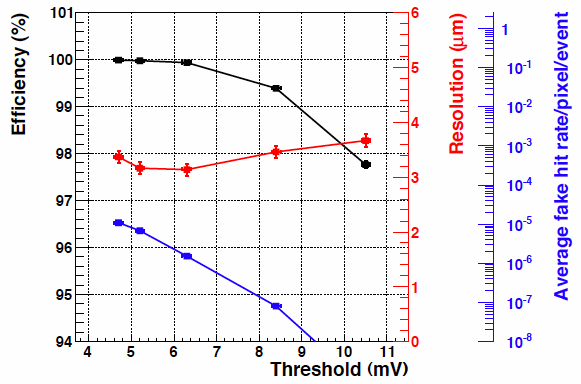
\includegraphics[width=0.8\textwidth]{Pictures/vxd/MIMOSA26_chip26_HR15_20deg}
      \caption{Plots representing the efficiency, the fake hit rate per pixel and the spatial resolution as a function of the discriminator threshold. This results were obtained with minimum ionising particles (pions of $120~\rm{GeV}$).}
      \label{fig:mi26Perf}
    \end{figure}

    The first full-scale digital sensor developed by the PICSEL group was the \gls{MIMOSA}-26.
    It was designed to equip the reference planes of the EUDET beam telescope and has been used since 2010 to build the PLUME prototypes.
    It is fabricated in the AMS $0.35~\rm{\mu m}$ technology and has a matrix containing approximately $6.6 \times 10^5$ pixels, distributed in $1152$ columns and $576$ rows.
    The pixel pitch is $18.4~\rm{\mu m}$ and the sensitive area corresponds to $21.2 \times 10.6~\rm{cm}^2$.
    The readout of the matrix is ensured by a rolling-shutter working at $80~\rm{MHz}$ frequency and the integration time is $115.2~\rm{\mu s}$.
    The signal produced by the charge collection inside the pixel is firstly amplified.
    Then, the \gls{CDS} technique is used to subtract successive frames before sending the signal to the bottom of the pixel array, where the signal processing circuitry is placed.
    Analog-to-digital conversion is done, coupled to a second double sampling, in order to reduce the \gls{FPN}.
    The output of the discriminators is then connected to a zero suppression logic, in which an output memory is duplicated to ensure a continuous readout.
    The signal is finally transmitted to the outside world.
    The performance obtained with a \gls{MIMOSA}-26 is shown in figure~\ref{fig:mi26Perf}.
    The architecture of the \gls{MIMOSA}-26 is represented by a block-diagram in figure~\ref{fig:archMi26}.
    The power consumption is $1.1~\rm{\mu W/pixel}$ and the sensor is thinned down to $50~\rm{\mu m}$ in order to minimise the multiple scattering inside the volume.

  \begin{figure}[!tbh]
    \hspace{-2cm}
    \centering
    \begin{subfigure}[t]{0.4\textwidth}
        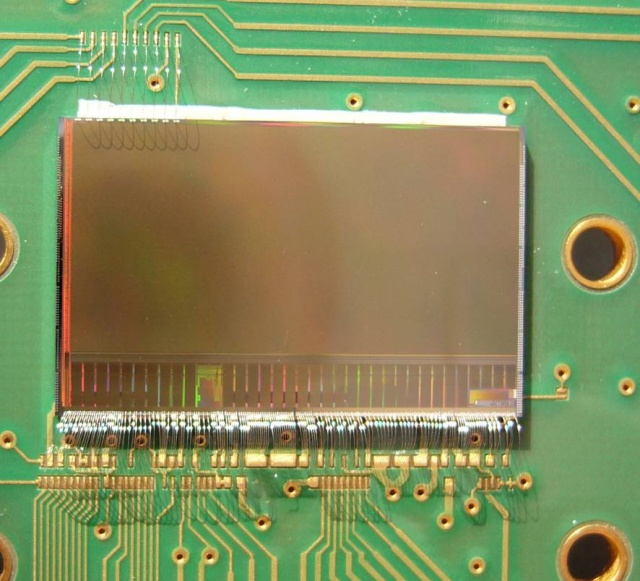
\includegraphics[width=0.95\textwidth]{Pictures/vxd/mi26.jpg}
        \caption{Picture of a MIMOSA-26 mounted on a PCB.}
        \label{fig:mi26}
    \end{subfigure}
    \qquad
     %add desired spacing between images, e. g. ~, \quad, \qquad, \hfill etc. 
      %(or a blank line to force the subfigure onto a new line)
    \begin{subfigure}[t]{0.4\textwidth}
        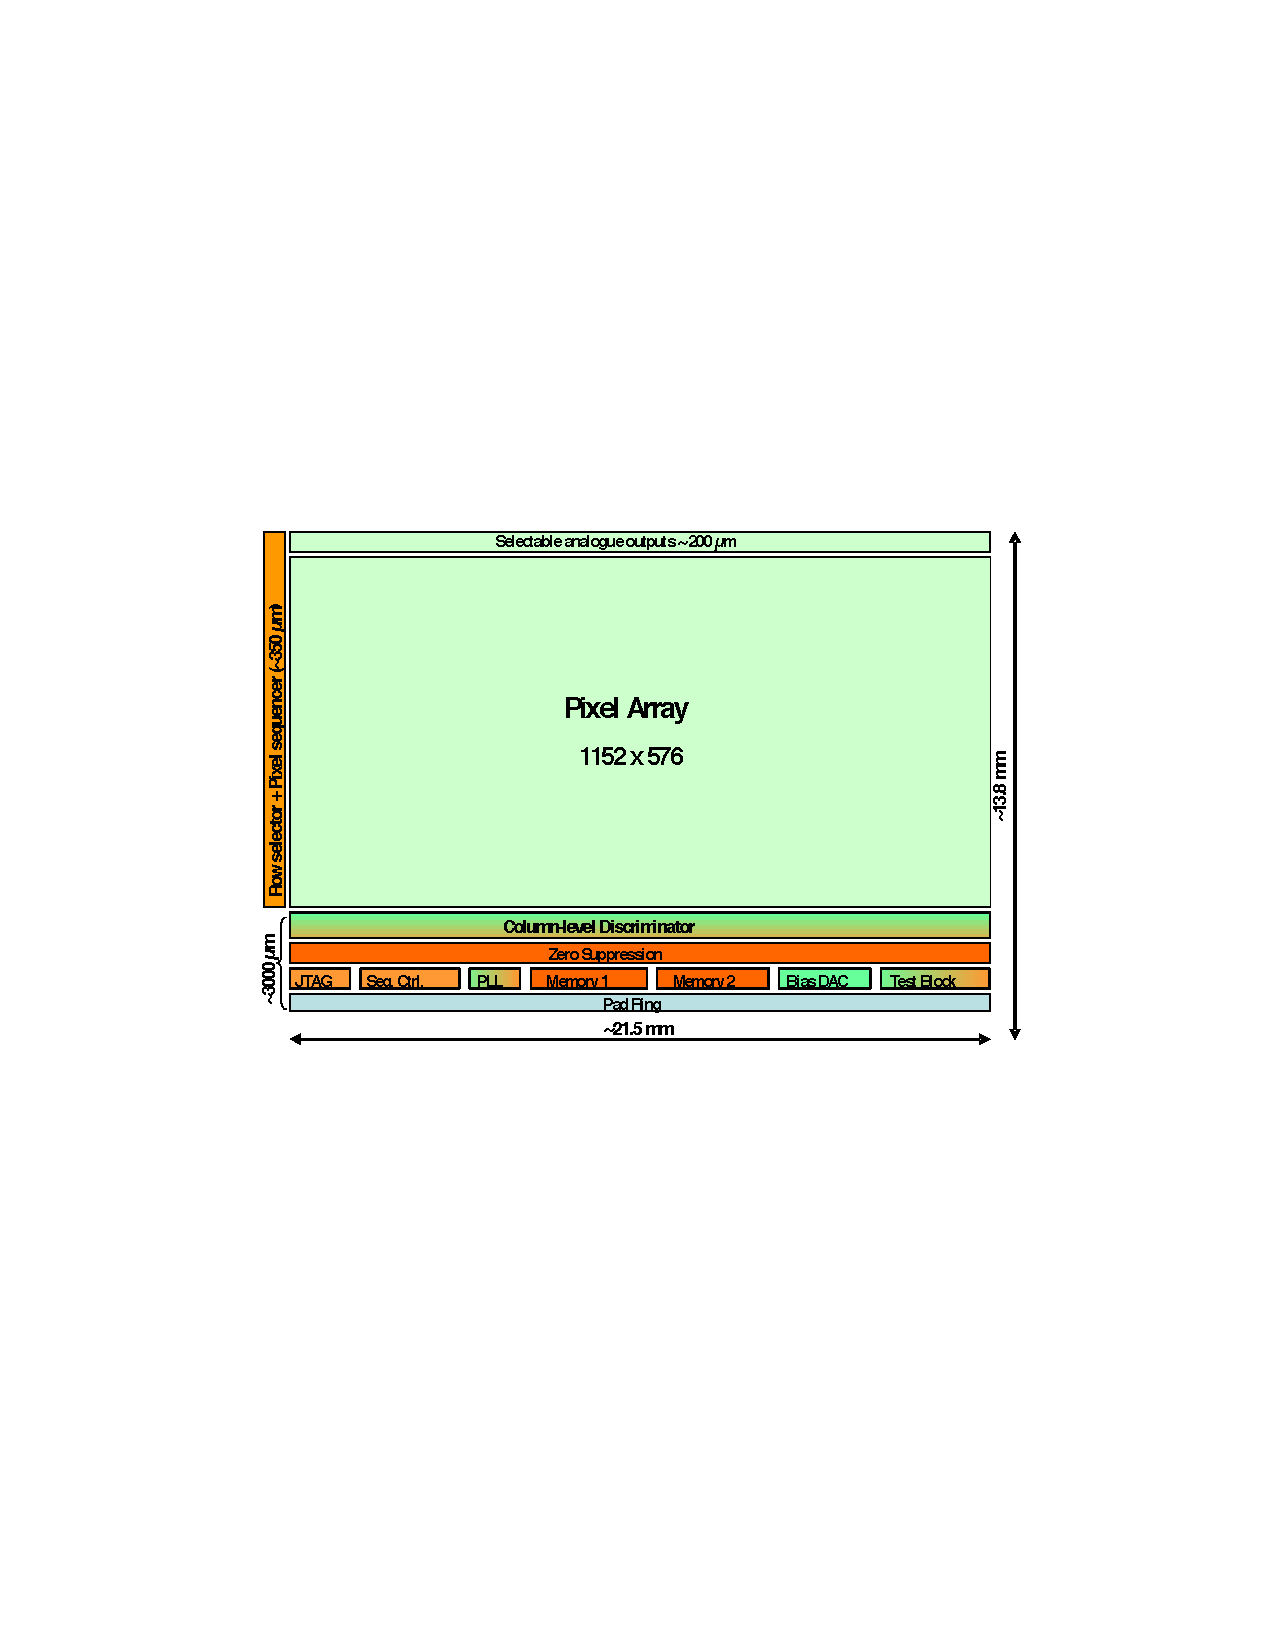
\includegraphics[width=1.35\textwidth]{Pictures/vxd/mi26_architecture.pdf}
        \caption{Layout of the MIMOSA-26 matrix.}
        \label{fig:archMi26}
    \end{subfigure}
    \caption{Block-diagram and a picture of the MIMOSA-26}\label{fig:Mi26}
    \end{figure}    

    The PICSEL group then developed digital output sensors for the pixel vertex detector at the STAR experiment at Brookhaven National Laboratory~\cite{1748-0221-7-01-C01102}\cite{1748-0221-10-03-C03026}.
    Figure~\ref{fig:Mi28} shows a half-section of the STAR vertex detector (figure~\ref{fig:vxdSTAR}) and a \gls{MIMOSA}-28 bonded on a PCB (figure~\ref{fig:ultimate}).
    They are based on the architecture of \gls{MIMOSA}-26 with some modifications.
    The matrix contains 960 columns and 928 rows for a pitch of $20.7 \times 20.7~\rm{\mu m}^2$.
    The sensitive area is $19.7 \times 19.2~\rm{cm}^2$, for an integration time of less than $200~\rm{\mu s}$.
    The sensor can reach a particle detection rate of $10^6~\rm{partices.cm}^{-2}\rm{.s}^{-1}$. 
    Finally, their power consumption is lower or equal to $150~\rm{mW.cm}^{-2}$.
    The spatial resolution obtained for ULTIMATE is less than $4~\rm{\mu m}$.

  \begin{figure}[!tbh]
    \centering
    \begin{subfigure}[t]{0.4\textwidth}
        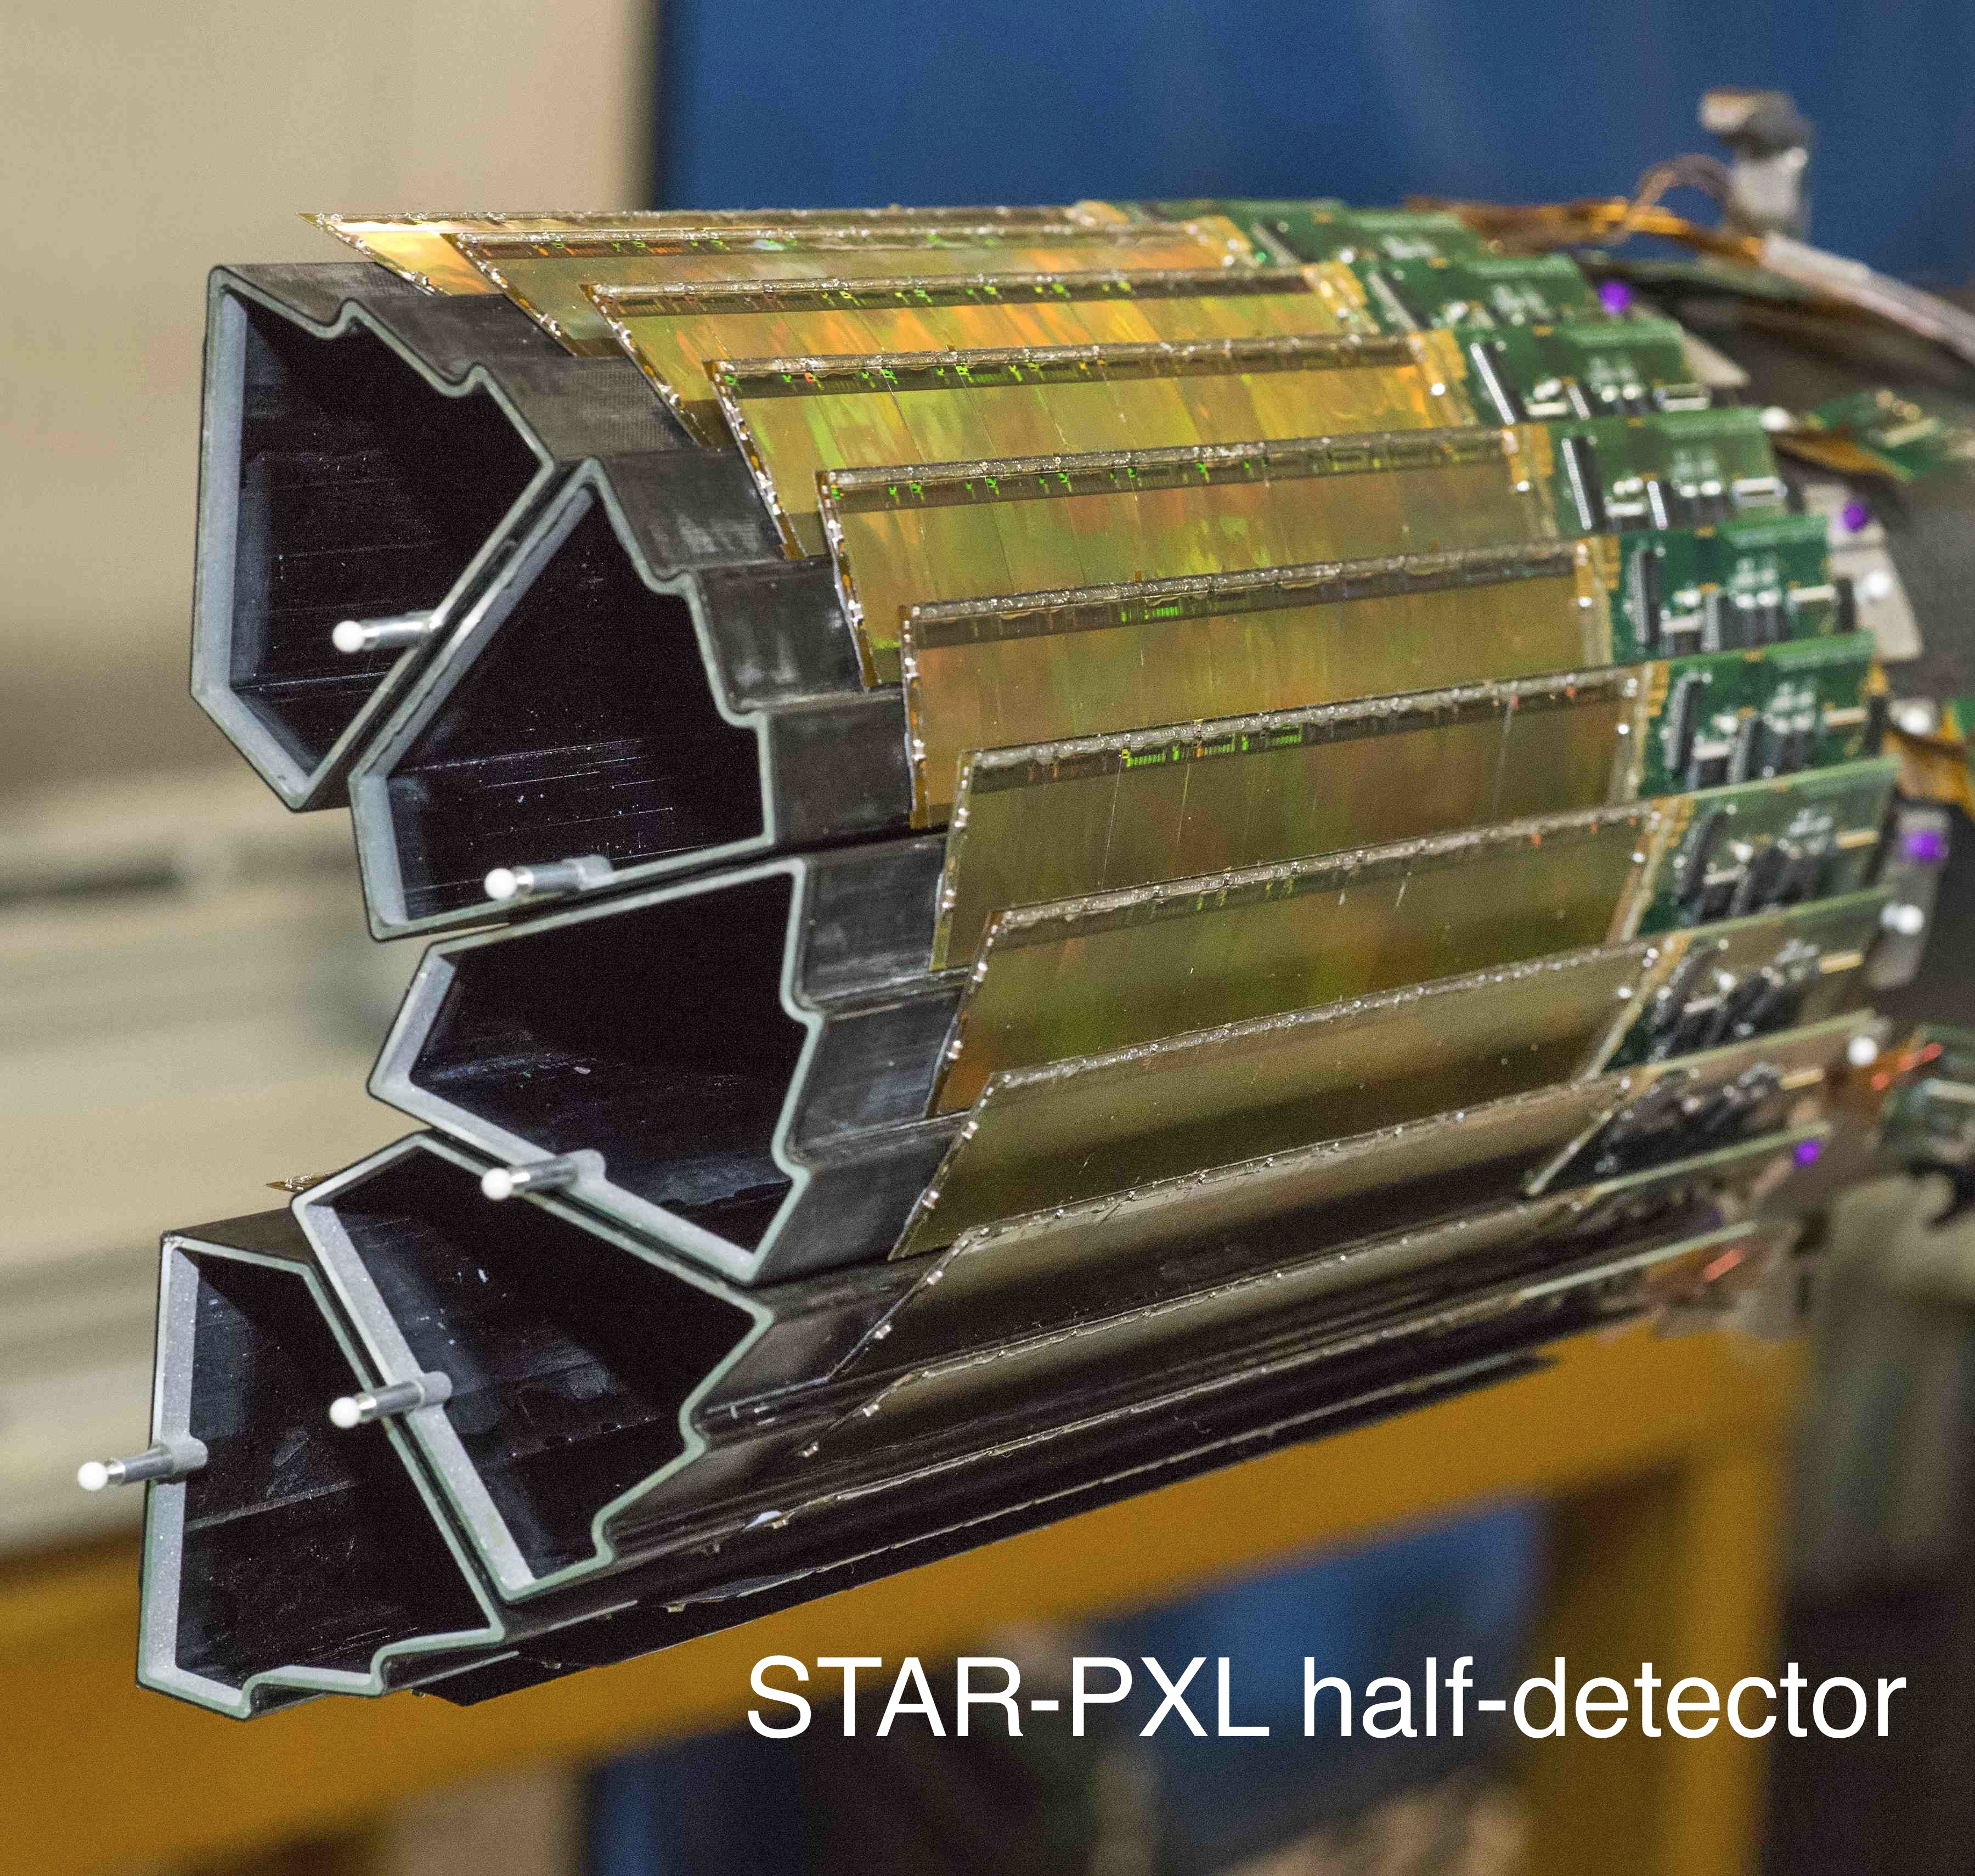
\includegraphics[width=\textwidth]{Pictures/vxd/pxlFinal_sideView_smallSize.jpg}
        \caption{Half part picture of the pixel vertex detector at STAR.}
        \label{fig:vxdSTAR}
    \end{subfigure}
    \qquad
     %add desired spacing between images, e. g. ~, \quad, \qquad, \hfill etc. 
      %(or a blank line to force the subfigure onto a new line)
    \begin{subfigure}[t]{0.4\textwidth}
        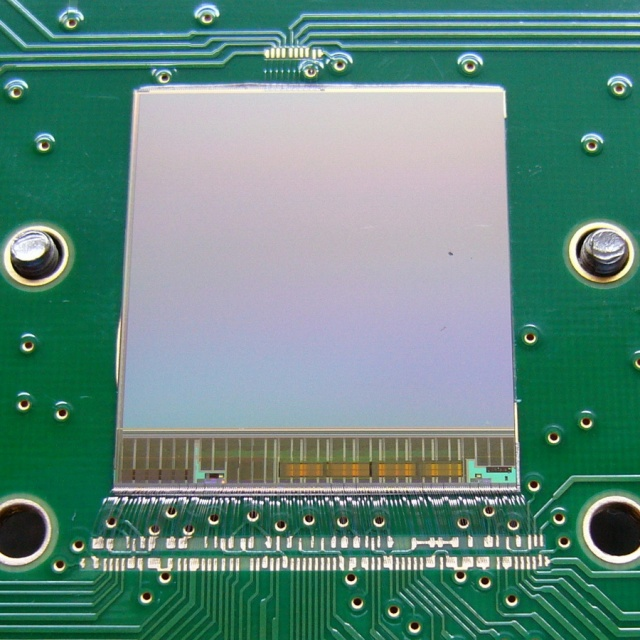
\includegraphics[width=0.95\textwidth]{Pictures/vxd/ultimate2.jpg}
        \caption{ULTIMATE chip mounted on a PCB. %The top wire bounds are used for a slow analog output dedicated to lab test, while the bottom ones are the wire bounds which control and read the sensor. }
        }
        \label{fig:ultimate}
    \end{subfigure}
    \caption{Pictures of the STAR vertex detector and an ULTIMATE chip}\label{fig:Mi28}
    \end{figure}    

    This chapter has depicted the purpose of the vertex detector for the \gls{ILD}.
    Different technologies were introduced, to focus specifically on the \gls{CMOS} sensors and their use in high-energy physics.
    The \gls{PLUME} collaboration aims to integrate \gls{MAPS} onto light double-sided ladders, in order to reach the requirements of the \gls{ILC}.
    The collaboration has performed different steps to produce the first full-scale ladder, which only have a material budget of $0.35~\%~\rm{X_0}$ and a spatial resolution better than $4~\rm{\mu m}$.
    The principle of \gls{CMOS} technology was presented. 
    The next chapter is focusing on the electrical validation of these sensors mounted onto a PLUME ladder.

    


